\documentclass[aps,preprint,preprintnumbers,nofootinbib,showpacs,prd]{revtex4-1}
\usepackage{graphicx,color}
\usepackage{caption}
\usepackage{subcaption}
\usepackage{amsmath,amssymb}
\usepackage{multirow}
\usepackage{amsthm}%        But you can't use \usewithpatch for several packages as in this line. The search 

\usepackage{cancel}

%%% for SLE
\usepackage{dcolumn}   % needed for some tables
\usepackage{bm}        % for math
\usepackage{amssymb}   % for math
\usepackage{multirow}
%%% for SLE -End

\usepackage{ulem}
\usepackage{cancel}

\usepackage{hyperref}
\usepackage{mathrsfs}
\usepackage[top=1in, bottom=1.25in, left=1.1in, right=1.1in]{geometry}

\usepackage{mathtools} % for \DeclarePairedDelimiter{\ceil}{\lceil}{\rceil}


\newcommand{\msout}[1]{\text{\sout{\ensuremath{#1}}}}


%%%%%% My stuffs - Stef
\newcommand{\lsim}{\mathrel{\mathop{\kern 0pt \rlap
  {\raise.2ex\hbox{$<$}}}
  \lower.9ex\hbox{\kern-.190em $\sim$}}}
\newcommand{\gsim}{\mathrel{\mathop{\kern 0pt \rlap
  {\raise.2ex\hbox{$>$}}}
  \lower.9ex\hbox{\kern-.190em $\sim$}}}

%
% Key
%
\newcommand{\key}[1]{\medskip{\sffamily\bfseries\color{blue}#1}\par\medskip}
%\newcommand{\key}[1]{}
\newcommand{\q}[1] {\medskip{\sffamily\bfseries\color{red}#1}\par\medskip}
\newcommand{\comment}[2]{{\color{red}{{\bf #1:}  #2}}}


\newcommand{\ie}{{\it i.e.} }
\newcommand{\eg}{{\it e.g.} }

%
% Energy scales
%
\newcommand{\ev}{{\,{\rm eV}}}
\newcommand{\kev}{{\,{\rm keV}}}
\newcommand{\mev}{{\,{\rm MeV}}}
\newcommand{\gev}{{\,{\rm GeV}}}
\newcommand{\tev}{{\,{\rm TeV}}}
\newcommand{\fb}{{\,{\rm fb}}}
\newcommand{\ifb}{{\,{\rm fb}^{-1}}}

%
% SUSY notations
%
\newcommand{\neu}{\tilde{\chi}^0}
\newcommand{\neuo}{{\tilde{\chi}^0_1}}
\newcommand{\neut}{{\tilde{\chi}^0_2}}
\newcommand{\cha}{{\tilde{\chi}^\pm}}
\newcommand{\chao}{{\tilde{\chi}^\pm_1}}
\newcommand{\chaop}{{\tilde{\chi}^+_1}}
\newcommand{\chaom}{{\tilde{\chi}^-_1}}
\newcommand{\Wpm}{W^\pm}
\newcommand{\chat}{{\tilde{\chi}^\pm_2}}
\newcommand{\smu}{{\tilde{\mu}}}
\newcommand{\smur}{\tilde{\mu}_R}
\newcommand{\smul}{\tilde{\mu}_L}
\newcommand{\sel}{{\tilde{e}}}
\newcommand{\selr}{\tilde{e}_R}
\newcommand{\sell}{\tilde{e}_L}
\newcommand{\smurl}{\tilde{\mu}_{R,L}}

\newcommand{\casea}{\texttt{IA}}
\newcommand{\caseb}{\texttt{IB}}
\newcommand{\casec}{\texttt{II}}

\newcommand{\caseasix}{\texttt{IA-6}}

%
% Greek
%
\newcommand{\es}{{\epsilon}}
\newcommand{\sg}{{\sigma}}
\newcommand{\dt}{{\delta}}
\newcommand{\kp}{{\kappa}}
\newcommand{\lm}{{\lambda}}
\newcommand{\Lm}{{\Lambda}}
\newcommand{\gm}{{\gamma}}
\newcommand{\mn}{{\mu\nu}}
\newcommand{\Gm}{{\Gamma}}
\newcommand{\tho}{{\theta_1}}
\newcommand{\tht}{{\theta_2}}
\newcommand{\lmo}{{\lambda_1}}
\newcommand{\lmt}{{\lambda_2}}
%
% LaTeX equations
%
\newcommand{\beq}{\begin{equation}}
\newcommand{\eeq}{\end{equation}}
\newcommand{\bea}{\begin{eqnarray}}
\newcommand{\eea}{\end{eqnarray}}
\newcommand{\ba}{\begin{array}}
\newcommand{\ea}{\end{array}}
\newcommand{\bit}{\begin{itemize}}
\newcommand{\eit}{\end{itemize}}

\newcommand{\nbea}{\begin{eqnarray*}}
\newcommand{\neea}{\end{eqnarray*}}
\newcommand{\nbeq}{\begin{equation*}}
\newcommand{\neeq}{\end{equation*}}

\newcommand{\no}{{\nonumber}}
\newcommand{\td}[1]{{\widetilde{#1}}}
\newcommand{\sqt}{{\sqrt{2}}}
%
\newcommand{\me}{{\rlap/\!E}}
\newcommand{\met}{{\rlap/\!E_T}}
\newcommand{\rdmu}{{\partial^\mu}}
\newcommand{\gmm}{{\gamma^\mu}}
\newcommand{\gmb}{{\gamma^\beta}}
\newcommand{\gma}{{\gamma^\alpha}}
\newcommand{\gmn}{{\gamma^\nu}}
\newcommand{\gmf}{{\gamma^5}}
%
% Roman expressions
%
\newcommand{\br}{{\rm Br}}
\newcommand{\sign}{{\rm sign}}
\newcommand{\Lg}{{\mathcal{L}}}
\newcommand{\M}{{\mathcal{M}}}
\newcommand{\tr}{{\rm Tr}}

\newcommand{\msq}{{\overline{|\mathcal{M}|^2}}}

%
% kinematic variables
%
%\newcommand{\mc}{m^{\rm cusp}}
%\newcommand{\mmax}{m^{\rm max}}
%\newcommand{\mmin}{m^{\rm min}}
%\newcommand{\mll}{m_{\ell\ell}}
%\newcommand{\mllc}{m^{\rm cusp}_{\ell\ell}}
%\newcommand{\mllmax}{m^{\rm max}_{\ell\ell}}
%\newcommand{\mllmin}{m^{\rm min}_{\ell\ell}}
%\newcommand{\elmax} {E_\ell^{\rm max}}
%\newcommand{\elmin} {E_\ell^{\rm min}}
\newcommand{\mxx}{m_{\chi\chi}}
\newcommand{\mrec}{m_{\rm rec}}
\newcommand{\mrecmin}{m_{\rm rec}^{\rm min}}
\newcommand{\mrecc}{m_{\rm rec}^{\rm cusp}}
\newcommand{\mrecmax}{m_{\rm rec}^{\rm max}}
%\newcommand{\mpt}{\rlap/p_T}

%%%song
\newcommand{\cosmax}{|\cos\Theta|_{\rm max} }
\newcommand{\maa}{m_{aa}}
\newcommand{\maac}{m^{\rm cusp}_{aa}}
\newcommand{\maamax}{m^{\rm max}_{aa}}
\newcommand{\maamin}{m^{\rm min}_{aa}}
\newcommand{\eamax} {E_a^{\rm max}}
\newcommand{\eamin} {E_a^{\rm min}}
\newcommand{\eaamax} {E_{aa}^{\rm max}}
\newcommand{\eaacusp} {E_{aa}^{\rm cusp}}
\newcommand{\eaamin} {E_{aa}^{\rm min}}
\newcommand{\exxmax} {E_{\neuo \neuo}^{\rm max}}
\newcommand{\exxcusp} {E_{\neuo \neuo}^{\rm cusp}}
\newcommand{\exxmin} {E_{\neuo \neuo}^{\rm min}}
%\newcommand{\mxx}{m_{XX}}
%\newcommand{\mrec}{m_{\rm rec}}
\newcommand{\erec}{E_{\rm rec}}
%\newcommand{\mrecmin}{m_{\rm rec}^{\rm min}}
%\newcommand{\mrecc}{m_{\rm rec}^{\rm cusp}}
%\newcommand{\mrecmax}{m_{\rm rec}^{\rm max}}
%%%song

\newcommand{\mc}{m^{\rm cusp}}
\newcommand{\mmax}{m^{\rm max}}
\newcommand{\mmin}{m^{\rm min}}
\newcommand{\mll}{m_{\mu\mu}}
\newcommand{\mllc}{m^{\rm cusp}_{\mu\mu}}
\newcommand{\mllmax}{m^{\rm max}_{\mu\mu}}
\newcommand{\mllmin}{m^{\rm min}_{\mu\mu}}
\newcommand{\mllcusp}{m^{\rm cusp}_{\mu\mu}}
\newcommand{\elmax} {E_\mu^{\rm max}}
\newcommand{\elmin} {E_\mu^{\rm min}}
\newcommand{\elmaxw} {E_W^{\rm max}}
\newcommand{\elminw} {E_W^{\rm min}}
\newcommand{\R} {{\cal R}}

\newcommand{\ewmax} {E_W^{\rm max}}
\newcommand{\ewmin} {E_W^{\rm min}}
\newcommand{\mwrec}{m_{WW}}
\newcommand{\mwrecmin}{m_{WW}^{\rm min}}
\newcommand{\mwrecc}{m_{WW}^{\rm cusp}}
\newcommand{\mwrecmax}{m_{WW}^{\rm max}}

\newcommand{\mpt}{{\rlap/p}_T}

%%%%%% END My stuffs - Stef

\newcommand{\dunno}{$ {}^{\mbox {--}}\backslash(^{\rm o}{}\underline{\hspace{0.2cm}}{\rm o})/^{\mbox {--}}$}

\DeclarePairedDelimiter{\ceil}{\lceil}{\rceil}
\DeclarePairedDelimiter{\floor}{\lfloor}{\rfloor}

\DeclareMathOperator{\re}{Re}


\begin{document}

\title{Jeffrey Stopple's Primer of Analytic Number Theory Book}
\bigskip
\author{Stefanus Koesno$^1$\\
$^1$ Somewhere in California\\ San Jose, CA 95134 USA\\
}
%
\date{\today}
%
\begin{abstract}
Very good book, had a lot of fun

\end{abstract}
%
\maketitle

\renewcommand{\theequation}{A.\arabic{equation}}  % redefine the command that creates the equation no.
\setcounter{equation}{0}  % reset counter 

Saw this somewhere, show that
%
\nbea
\sum_{n=1}^\infty \frac{2}{n(n+1)} & = & 1+\frac{1}{3}+\frac{1}{6}+\frac{1}{10}+\ldots = 2
\neea
%
historically this was first proved by Pietro Mengoli in 1650, the real gist of the story is that Mengoli couldn't deduce the value of the sum $\sum_n 1/n^2$ which is similar to the one above (this quadratic harmonic series was finally solved by Euler, neither Leibnitz nor Bernoulli could do it). So back to the original problem, my approach was to split $\frac{2}{n(n+1)}$ into a sum of two fractions
%
\nbea
\frac{2}{n(n+1)} & = & \frac{A}{n}+\frac{B}{n+1} \\
& = & \frac{An+A+Bn}{n(n+1)}
\neea
%
this means that $A = 2$ and $B=-2$ and thus the series can be written as
%
\nbea
\sum_{n=1}^\infty \frac{2}{n(n+1)} & = & \sum_{n=1}^\infty \left(\frac{2}{n} - \frac{2}{n+1}\right) \\
& = & \left(\frac{2}{1} - \frac{2}{2}\right) + \left(\frac{2}{2} - \frac{2}{3}\right) + \left(\frac{2}{3} - \frac{2}{4}\right) + \left(\frac{2}{4} - \right. \ldots \\
& = & \frac{2}{1} + \left( - \frac{2}{2} + \frac{2}{2} \right) + \left( - \frac{2}{3}+ \frac{2}{3}\right) + \left( - \frac{2}{4}+ \frac{2}{4}\right) + \ldots \\
& = & 2
\neea
%
so the series more or less ``telescopes'' and we are left with just the first term although I believe the method above is not legit as we turned an (absolutely?) convergent series into a conditionally convergent series? \dunno ~~~but to then again it might still be ok because if we denote
%
\nbea
H_n & = & \frac{2}{n} -\frac{2}{n+1} \\
\to S(k) & = & \sum_{n=1}^k H_n \\
& = & \frac{2}{1} - \frac{2}{k+1}
\neea
%
and if we take the limit $k\to\infty$
%
\nbea
\lim_{k\to\infty} S(k) & = & \frac{2}{1} - \frac{2}{\infty} \\
& = & 2
\neea
%
the only trick remaining is showing that
%
\nbea
\sum_{n=1}^\infty \frac{2}{n(n+1)} & = & \lim_{k\to\infty} S(k)
\neea
%
which can be shown by noting that if the sum is not infinite the two agree, \ie
%
\nbea
\sum_{n=1}^k \frac{2}{n(n+1)} & = & S(k)
\neea
%
so if we take both sides to infinity we get
%
\nbea
\to \lim_{k\to\infty}\sum_{n=1}^k \frac{2}{n(n+1)} & = & \lim_{k\to\infty} S(k) \\
\sum_{n=1}^\infty \frac{2}{n(n+1)} & = & 2
\neea
%
sounds a lot like a roundabout way of saying the same thing LOL \dunno

-=-=-=-=-=-=-=-=--=-=-=-=-=-=-=-=--=-=-=-=-=-=-=-=--=-=-=-=-=-=-=-=--=-=-=-=-=-=-=-=--=-=-=-=-=

{\bf Exercise 1.2.1}, Page 12, Imitate this argument to get a formula for the hexagonal numbers $h(n)$.

A triangular number, $t_n$ is a number where $t_1=1$ and $t_2 = 3$ and because it's 3 it's a triangular number, the explicit formula is
%
\nbea
t_n & = & \frac{n(n+1)}{2}
\neea
%
which is just $1 + 2 + \ldots + n$.

For the hexagonal number we have $\Delta^2h(n) = 6-2 = 4$ and so $\Delta h(n) = 4n + C$ such that
%
\nbea
\Delta^2h(n) = \Delta(\Delta h(n)) = \Delta(4n+C) = (4(n+1)+C) - (4n+C) = 4
\neea
%
This means that $h(n)$ should contain $Cn+D$ such that $\Delta h(n) = (C(n+1) + D) - (Cn+D) = C$ but this should not be the only term $h(n)$ contains, it should also contain a term whose difference is $4n$ because $\Delta h(n)$ contains $4n$ and that is provided by
%
\nbea
\Delta(4t(n-1)) = 4t(n) - 4t(n-1) = 4\frac{n(n+1)}{2} - 4\frac{n(n-1)}{2} = 4n
\neea
%
so
%
\nbea
h(n) = 4t(n-1) + Cn + D = 2n(n-1) + Cn + D
\neea
%
applying initial conditions $h(1) = 1$ and $h(2) = 6$
%
\nbea
0 + C + D & = & 1 \\
4 + 2C + D & = & 6
\neea
%
giving $C=1$ and $D=0$, so
%
\nbea
h(n) & = & 2n(n-1) + n = n(2n-1)
\neea
%
This seems to be correct since it gives
%
\nbea
\begin{array}{r c c c c c c c c c}
h(n): & 1 & 6 & 15 & 28 & 45 & 66 & 91 & 120 & \ldots, \\
\Delta h(n): & 5 & 9 & 13 & 17 & 21 & 25 & 29 & 33 & \ldots, \\
\Delta^2h(n): & 4 & 4 & 4 & 4 & 4 & 4 & 4 & 4 & \ldots .
\end{array}
\neea
%
and in general $\ldots$

{\bf Exercise 1.2.4}, Page 14, find a formula for polygonal numbers with $a$ sides, for any $a$, \ie a function $f(n)$ with
%
\nbea
\Delta^2f(n) = a - 2, & ~~~~~~~~~~~~ & {\rm with~} f(1) = 1 {\rm ~and~} f(2) = a.
\neea
%

Using the result from Exercise 1.2.1 the generic formula we have is
%
\nbea
f(n) = (a-2)t(n-1) + Cn + D = (a-2)n(n-1)/2 + Cn + D
\neea
%
applying initial conditions
%
\nbea
0 + C + D & = & 1 \\
(a-2) + 2C + D & = & a
\neea
%
which means it's actually independent of $a$, interesting, and therefore $C=1$ and $D=0$ all the time $\ldots$ and therefore
%
\nbea
f(n) & = & n\left\lbrack\left(\frac{a}{2}-1\right)n - \frac{a}{2} + 2\right\rbrack
\neea
%
the good thing about this is that it works for {\bf any} $a$, zero, positive and negative.

{\bf Exercise 1.2.5}, Page 16, verify that
%
\nbea
n^{\underline 1} + 3n^{\underline 2} + n^{\underline 3} & = & n^3
\neea
%
Now use this fact to find formulas for
%
\nbea
\sum_{0\le k <n+1} k^3.
\neea
%

%
\nbea
n^{\underline 1} & = & n\\
3n^{\underline 2} & = & 3n(n-1) \\
& = & 3n^2 - 3n \\
n^{\underline 3} & = & n(n-1)(n-2) \\
& = & n^3 - 3n^2 + 2n
\neea
%
so it's obvious if we sum them we get $n^3$, now we need to ``integrate'' these things
%
\nbea
\Sigma (n^{\underline 1} + 3n^{\underline 2} + n^{\underline 3}) & = & \frac{n^{\underline 2}}{2} + \bcancel{3}\frac{n^{\underline 3}}{\bcancel{3}} + \frac{n^{\underline 4}}{4}
\neea
%
using this in the big sum we get
%
\nbea
\sum_{0\le k <n+1} k^3 & = & \left.\Sigma(n^{\underline 1} + 3n^{\underline 2} + n^{\underline 3})\right|_0^{n+1} \\
& = & \left.\frac{n^{\underline 2}}{2} + n^{\underline 3} + \frac{n^{\underline 4}}{4}\right|_0^{n+1} \\
& = & \frac{(n+1)^{\underline 2}}{2} + (n+1)^{\underline 3} + \frac{(n+1)^{\underline 4}}{4} \\
& = & \frac{(n+1)n}{2} + (n+1)n(n-1) + \frac{(n+1)n(n-1)(n-2)}{4} \\
& = & \frac{n(n+1)\{2 + 4(n-1) + (n-1)(n-2)\}}{4} \\
& = & \frac{n^2(n+1)^2}{4}
\neea
%

{\bf Exercise 1.2.12}, Page 21, Use the fact that if $\Delta f(k) = g(k)$ and $a$ is any constant, then $\Delta (f(k+a)) = g(k+a)$, and the fact that $2(k-1)^{\underline {-2}} = 1/t_k$ to find the sum of the reciprocals of the first $n$ triangular numbers
%
\nbea
\frac{1}{t_1} + \frac{1}{t_2} + \ldots + \frac{1}{t_n}.
\neea
%
Next compute
%
\nbea
\frac{1}{T_1} + \frac{1}{T_2} + \ldots + \frac{1}{T_n},
\neea
%
the sum of the reciprocals of the first $n$ tetrahedral numbers.

So what we want is
%
\nbea
\sum_{1\le k < n+1} \frac{1}{t_k} & = & \left.\Sigma \frac{1}{t_k} \right |_{1}^{n+1} \\
& = & \left.\Sigma 2(k-1)^{\underline{-2}} \right |_{1}^{n+1} \\
& = & \left.\Sigma \frac{2(k-1)^{\underline{-1}}}{-2+1} \right |_{1}^{n+1} \\
& = & -2 \left \lbrack (n)^{\underline{-1}} - 0^{\underline{-1}}\right\rbrack \\
& = & -2\left\lbrack\frac{1}{(n+1)} - \frac{1}{0+1}\right\rbrack \\
& = & \frac{2n}{n+1}
\neea
%
the thing to note here is that $0^{\underline{-1}}$ is {\bf not} zero it is actually $1/(0+1) = 1$. For the tetrahedral numbers we know that it is given in Eq. 1.4 and 1.5
%
\nbea
T_n & = & \frac{n(n+1)(n+2)}{6} \\
\to \frac{1}{T_n} & = & 6~\frac{1}{n(n+1)(n+2)}\\
& = & 6 (n-1)^{\underline{-3}}
\neea
%
so the sum is also pretty much the same
%
\nbea
\sum_{1\le k < n+1} \frac{1}{T_k} & = & \left.\Sigma \frac{1}{T_k} \right |_{1}^{n+1} \\
& = & \left.\Sigma 6(k-1)^{\underline{-3}} \right |_{1}^{n+1} \\
& = & \left.\Sigma \frac{6(k-1)^{\underline{-2}}}{-3+1} \right |_{1}^{n+1} \\
& = & -3 \left \lbrack (n)^{\underline{-2}} - 0^{\underline{-2}}\right\rbrack \\
& = & -3\left\lbrack\frac{1}{(n+1)(n+2)} - \frac{1}{(0+1)(0+2)}\right\rbrack \\
& = & \frac{3(n^2+3n)}{2(n+1)(n+2)}
\neea
%

{\bf Exercise 1.2.13}, Page 23, Use Summation by Parts and the Fundamental Theorem to compute $\sum_{0\le k<n}H_k$. (Hint: You can write $H_k = H_k \cdot 1 = H_k\cdot k^{\underline 0}$.) Your answer will have Harmonic numbers in it of course.

%
\nbea
\Sigma H_k & = & \Sigma (H_k \cdot 1) = \Sigma (H_k\cdot k^{\underline 0})
\neea
%
I don't know how to integrate $H_k$ (since that is the question we are trying to answer here) but I know how to differentiate it, the derivative is just $k^{\underline{-1}}$ so we'll take $u = H_k$ such that $\Delta u = k^{\underline{-1}}$ and so we'll take $\Delta v = k^{\underline 0}$ such that $v = k^{\underline 1}$.

Next we need $\Sigma(\Delta u\cdot Ev)$
%
\nbea
\Sigma(\Delta u\cdot Ev) & = & \Sigma(k^{\underline{-1}} \cdot (k+1)^{\underline 1}) \\
& = & \Sigma\left(\frac{1}{\bcancel{(k+1)}}\cdot \bcancel{(k+1)}k \right) \\
& = & \frac{k^{\underline 2}}{2}
\neea
%
so we have
%
\nbea
\Sigma (u\cdot\Delta v) & = & uv - \Sigma(\Delta u\cdot Ev) \\
\to \Sigma (H_k\cdot k^{\underline 0}) & = & H_k k^{\underline 1} - \frac{k^{\underline 2}}{2}
\neea
%
to verify let's differentiate it
%
\nbea
\Delta\left(H_k k^{\underline 1} - \frac{k^{\underline 2}}{2}\right) & = & k^{\underline {-1}}(k+1)^{\underline 1} + H_k k^{\underline 0} - k^{\underline 1} \\
& = & \frac{(k+1)k}{k+1} + H_k - k \\
& = & H_k
\neea
%
note that the product rule here is different, there's a shift involved, see Page 22, and therefore
%
\nbea
\sum_{0 \le k < n} H_k\cdot k^{\underline 0} & = & \left.\Sigma(u\cdot\Delta v)\right|_0^{n} \\
& = & \left. \left( H_k k^{\underline 1} - \frac{k^{\underline 2}}{2}\right)\right |_0^n\\
& = & n\left(H_n - \frac{n-1}{2}\right)
\neea
%

{\bf Exercise 1.2.14}, Page 23, Use Summation by Parts and the Fundamental Theorem to compute $\sum_{0\le k <n}k2^k$. (Hint: You need the first part of Exercise 1.2.9.)

The thing to note here is that $2^k$ is like $e$ its derivative is itself
%
\nbea
\Delta 2^k & = & 2^{k+1} - 2^k \\
& = & 2^k
\neea
%
so we will want this to be $\Delta v = 2^k$ such that $v = 2^k$ and $u = k = k^{\underline 1}$ such that $\Delta u = k^{\underline 0} = 1$ and so
%
\nbea
\Sigma(u\cdot \Delta v) & = & uv - \Sigma(\Delta u\cdot Ev) \\
& = & k^{\underline 1} 2^k - \Sigma\left(k^{\underline 1} 2^{k+1}\right) \\
& = & k2^k - \Sigma(2^{k+1}) \\
& = & k2^k - 2^{k+1} \\
& = & 2^k(k - 2)
\neea
%
to verify let's differentiate the above
%
\nbea
\Delta\left\{ 2^k(k - 2) \right\} & = & 2^k ((k+1)-2) + 2^k \\
& = & k2^k
\neea
%
so it's correct and again the thing to note is that the product rule here now involves a shift, moving on
%
\nbea
\sum_{0\le k <n} k2^k & = & \left. \left( 2^k(k - 2) \right) \right |_0^n \\
& = & 2^n(n-2) - (-2) \\
& = & 2^n(n-2) + 2
\neea
%

-=-=-=-=-=-=-=-=--=-=-=-=-=-=-=-=--=-=-=-=-=-=-=-=--=-=-=-=-=-=-=-=--=-=-=-=-=-=-=-=--=-=-=-=-=

{\bf Exercise 2.1.7}, Page 30, we know that $6=2^1\cdot3$ and $28=2^2\cdot 7$ are perfect numbers. The next ones are $496=2^4\cdot31$ and $8128=2^6\cdot127$ (check this!). What is the pattern in $3,7,31,127,\ldots$ ? What is the pattern in the exponents $1,2,4,6,\ldots$ ? Try to make a conjecture about perfect numbers. Euclid, in his {\it Elements}, proved a general theorem about perfect numbers around the year 300 B.C.

%
\nbea
3 & = & 2^2 - 1 \\
7 & = & 2^3 - 1 \\
31 & = & 2^5 - 1\\
127 & = & 2^7 - 1
\neea
%
so the exponents are $2,3,5,7$ which are all primes and are all one more that the $1,2,4,6$ so it looks like the formula for even perfect numbers are
%
\nbea
2^{p-1}\cdot (2^p - 1)
\neea
%
where $p$ is prime.

{\bf Exercise 2.1.8}, Page 30, \#2 and \#3 are the interesting ones since the exponents of the $2^p-1$ are 11 and 13 and they are both prime so $2^{10}(2^{11}-1)$ and $2^{12}(2^{13}-1)$ are also prime, let's start with \#2

%
\nbea
2096128 & = & 2^{10}(2^11-1) = 2^{10}\cdot 23 \cdot 89 \\
\to \sigma(2096128) & = & \sigma(2^{10}) \sigma(23) \sigma(89) \\
& = & (2^11-1) (23+1)(89+1) \\
& = & 4421520 \\
\to s(2096128) & = & \sigma(2096128) - 2096128  = 2325392\\
& \neq & 2096128
\neea
%
so even though 11, the exponent of $2^{11}-1$ is prime, $2^{10}(2^{11}-1)$ is not perfect, while
%
\nbea
33550336 & = & 2^{12}(2^{13}-1) = 2^{12} \cdot 8191 \\
\to \sigma(33550336) & = & \sigma(2^{12})\sigma(8191) \\
& = & (2^{13}-1)(8191+1) \\
& = & 8191\cdot(8191+1) \\
& = & 67100672 \\
\to s(33550336) & = & \sigma(33550336) - 33550336 = 33550336
\neea
%
so it is a perfect number, thus the formula has to be correctec to only include $2^p-1$ that is prime (and $p$ itself is also prime)

{\bf Exercise 2.1.12}, Page 31, there is an interesting theorem about perfect numbers and sums of cubes. For example,
%
\nbea
28 = 1^3 + 3^3
\neea
%
Try to make a conjecture about what is true. Ignore the first perfect number, 6; it doesn't fit the pattern.
%
\nbea
28 & = & 1^3 + 3^3\\
496 & = & 1^3 + 3^3 + 5^3 + 7^3\\
8128 & = & 1^3 + 3^3 + 5^3 + 7^3 + 9^3 + 11^3 + 13^3 + 15^3
\neea
%
the pattern is given by the next exercise

{\bf Exercise 2.1.12}, Page 31,
%
\nbea
1^3 + 3^3 + 5^3 + \ldots + (2N-1)^3 & = & \left(1^3 + 2^3 + 3^3 + \ldots + (2N)^3\right) - \left(2^3+4^3+6^3 + \ldots+(2N)^3\right) \\
& = & \frac{(2N)^2(2N+1)^2}{4} - 2^3\left(1^3 + 2^3 + 3^3 + \ldots+N^3\right) \\
& = & \frac{4N^2(2N+1)^2}{4} - 2^3 \frac{N^2(N+1)^2}{4} \\
& = & N^2(2N+1)^2 - 2N^2(N+1)^2 \\
& = & N^2 \left( 4N^2 + 4N + 1 - 2N^2 - 4N - 2\right) \\
& = & N^2(2N^2-1)
\neea
%
so $N=2^{(p-1)/2}$ where $p$ is prime and $2^p-1$ is also prime

{\bf Exercise 2.1.16}, Page 33, Suppose $m$ and $n$ are integers such that $\sigma(m) = m + n = \sigma(n)$. What can you say is true about $s(m)$ and $s(n)$?
%
\nbea
s(m) & = & \sigma(m) - m \\
& = & m+n-m \\
s(m)& = & n
\neea
%
and
%
\nbea
s(n) & = & \sigma(n) - n\\
& = & m+n-n \\
s(n)& = & m
\neea
%
so a pair of amicable numbers $m$ and $n$ are those such that $s(m)=n$ and $s(n) = m$ and therefore $\sigma(m)=\sigma(n) = m+n$.

\bigskip
\underline{\textbf{\textit{Chapter 3}}}
\bigskip

Lessons from Chapter 3
%
\bit
\item Area is equal to length if the width is one, this is the trick used over and over, once you morphed length into area you can use integrals
\eit

\bigskip
\underline{\textbf{\textit{Chapter 4}}}
\bigskip

His notion of average order is slightly different than that of Apostol's

{\bf Exercise 4.2.4}, Page 76, the differences are
%
\nbea
\frac{1}{3} - \frac{27}{82} & = & 0.0040650406504065040650406504065 \\
\frac{27}{82} - \frac{15}{46} & = & 0.00318133616118769883351007423118 \\
\frac{15}{46} - \frac{12}{37} & = & 0.00176263219741480611045828437133
\neea
%
very small indeed, roughly one part in a thousand

{\bf Page 80}, {\bf Corollary}. {\it The average order of $\sigma(n)$ is $\zeta(2)n$.} Note that here he's talking about average order quite differently from Apostol, his reasoning here is since
%
\nbea
\sum_{k=1}^n \sigma(k) &\sim& \zeta(2)\frac{n^2}{2} \\
\sum_{k=1}^n \zeta(2) k &\sim& \zeta(2)\frac{n^2}{2} \\
\to \sum_{k=1}^n \sigma(k) &\sim& \sum_{k=1}^n \zeta(2) k
\neea
%
so since both sides are summed exactly the same each term as the same average order? \dunno

\bigskip
\underline{\textbf{\textit{Interlude 1}}}
\bigskip

{\bf Exercise I1.3.4}, Page 95, from the {\it definition} of $\log(x)$ as an integral over $1/t$
%
\nbea
\log(xy) & = & \int_1^{xy} \frac{1}{t} dt \\
& = & \int_1^x \frac{1}{t} dt + \int_x^{xy} \frac{1}{t} dt \\
& = & \log(x) + \int_x^{xy} \frac{1}{t} dt
\neea
%
The second term in the RHS can be massaged using the usual change of variable $s = xt$ such that $t = s/x$ and $dt = ds/x$ and so
%
\nbea
\int_x^{xy} \frac{1}{t} dt & = & \int_1^{y} \frac{\bcancel{x}}{s} \frac{ds}{\bcancel{x}} \\
& = & \log(y)
\neea
%
and so $\log(xy) = \log(x) + \log(y)$, we can actually do the change of variable in a slightly different way
%
\nbea
\int_x^{xy} \frac{1}{t} dt & = & \int_1^{y} \frac{x}{x}\times\frac{1}{t} dt \\
& = & \int_x^{xy} \frac{1}{(xt)} d(xt), ~~~~~ s=xt \\
& = & \int_1^{y} \frac{1}{s} ds \\
\neea
%
it was OK to do that because here $x$ is constant w.r.t the integration. A more interesting thing would be $\log(x/y)$ in this case
%
\nbea
\log(x/y) & = & \int_1^{x/y} \frac{1}{t} dt \\
& = & \int_1^{x} \frac{1}{t} dt - \int_{x/y}^{x} \frac{1}{t} dt
\neea
%
here we have a subtraction because $x/y < x$, the next steps are the same as previous case's.

\bigskip
\underline{\textbf{\textit{Chapter 5}}}
\bigskip

{\bf Page 107}, lower half of page, nearing the funny trick to prove the Theorem we have
%
\nbea
\pi(2n+1) & < & 2\frac{2n+1}{\log(2n)} \\
& < & 2\frac{2n+1}{\log(2n+1)}\frac{\log(2n+1)}{\log(2n)}
\neea
%
and for $n=30$, $\frac{\log(2n+1)}{\log(2n)} = 1.00403710574428$ so we can just adjust the constant 2 to $2.008\ldots$ or something :) and we can certainly do approximation this way as well
%
\nbea
\frac{\log(2n+1)}{\log(2n)} & = & \frac{\log(2n)+\log(1+1/2n)}{\log(2n)} \\
& \approx & 1
\neea
%
But actually if you numerically calculate $3.39 \frac{n}{\log(n)}+1$ and $2\frac{2n+1}{\log(2n+1)}$ starting at $n=67$, $3.39 \frac{n}{\log(n)}+1 < 2\frac{2n+1}{\log(2n+1)}$ and we can sort of prove this. 

Even simpler, we can compare $4n/\log(2n)$ and $2(2n+1)/\log(2n+1)$, let's take their ratio
%
\nbea
\frac{2(2n+1)/\log(2n+1)}{4n/\log(2n)} & = & \frac{4n+2}{\log(2n+1)}\frac{\log(2n)}{4n}\\
& = & \frac{4n+2}{4n} \frac{\log(2n)}{\log(2n+1)} \\
& = & \left(1 + \frac{1}{2n}\right)\frac{\log(2n)}{\log(2n) + \log\left(1 + \frac{1}{2n}\right)} \\
& = & \left(1 + \frac{1}{2n}\right) \frac{1}{1 + \frac{\log\left(1 + \frac{1}{2n}\right)}{\log(2n)}}
\neea
%
if $\frac{\log\left(1 + \frac{1}{2n}\right)}{\log(2n)}$ is smaller than $\frac{1}{2n}$ than the whole ratio is greater than one and $2(2n+1)/\log(2n+1) > 4n/\log(2n)$. So again we take the ratio
%
\nbea
\frac{1/2n}{\log\left(1 + \frac{1}{2n}\right)/\log(2n)} & = & \frac{\log(2n)}{2n\log\left(1 + \frac{1}{2n}\right)} \\
& = & \frac{\log(2n)}{\log\left(1 + \frac{1}{2n}\right)^{2n}}
\neea
%
Now
%
\nbea
\lim_{n\to\infty} \left(1 + \frac{1}{n}\right)^{n}
\neea
%
is the definition of $e$ and it takes its minimum value when $n=1$ and as $n$ grows it grows bigger, we can see this using the binomial expansion (there's a derivation showing exactly this by Gilles Cazelais and I'll reproduce it here), first denote
%
\nbea
t_n & = & \left(1+\frac{1}{n}\right)^n
\neea
%
and so
%
\nbea
t_n  & = & \sum_{k=0}^n {n \choose k}\left(\frac{1}{n}\right)^k \\
& = & 1 + n\left(\frac{1}{n}\right) + \frac{n(n-1)}{2!}\left(\frac{1}{n^2}\right)+ \frac{n(n-1)(n-2)}{3!}\left(\frac{1}{n^3}\right) + \ldots + \frac{n(n-1)(n-2)\ldots 1}{n!}\left(\frac{1}{n^n}\right) \\
& = & 1 + 1 + \frac{1}{2!}\left(1-\frac{1}{n}\right) + \frac{1}{3!}\left(1-\frac{1}{n}\right)\left(1-\frac{2}{n}\right) + \ldots + \frac{1}{n!}\left(1-\frac{1}{n}\right)\left(1-\frac{2}{n}\right)\ldots \left(1-\frac{n-1}{n}\right)
\neea
%
the two key observations here are
%
\nbea
0 < \left(1-\frac{k}{n}\right) <1, & {\rm ~~~~~~~and~~~~~~~} & \left(1-\frac{k}{n}\right) < \left(1-\frac{k}{n+1}\right)
\neea
%
this means that $t_n < t_{n+1}$, in our case we only care about even $n$'s but the conclusion is the same $t_{2n}<t_{2(n+1)}$.

So when $n < \infty$, $\log\left(1 + \frac{1}{2n}\right)^{2n} < \log(e) < 1$. Now we need the numerator to be $>1$ so we need to take $n\ge2$ to ensure $2n > e$ and this is good enough for us.

So in conclusion, $\frac{1/2n}{\log\left(1 + \frac{1}{2n}\right)/\log(2n)} > 1$ means that $\left(1 + \frac{1}{2n}\right) \frac{1}{1 + \log\left(1 + \frac{1}{2n}\right)/\log(2n)} > 1$ and that finally means that $2(2n+1)/\log(2n+1) > 4n/\log(2n)$ and since $3.39 \frac{n}{\log(n)}+1 < 4n/\log(2n)$ it also means that $3.39 \frac{n}{\log(n)}+1 < 2(2n+1)/\log(2n+1)$.



{\bf Page 108}, Theorem that says
%
\nbea
\frac{1}{2}\frac{x}{\log(x)} < \pi(x)
\neea
%
for $x\ge15$. In fact we can say that this is true for $x\ge3$, 15 numbers are not too much to check so if you just calculate all 15 of them you'll see that this inequality holds for $x\ge3$ \dunno

{\bf Page 108}, Lemma, this is actually Theorem 3.14 of Apostol, so here's I replicate my own explanation of why this is true, visually we can see it below with an example for  $\alpha(p)$ with $x=10$ and $p=2$, each column shows the number of 2's in each number (we only consider even numbers here obviously)
%
\nbea
\begin{array}{c c c c c l}
   &    &   & 2  &  & \longrightarrow x/p^3 = 10/2^3 = 1 {\rm~factor~of~} 2\\
   & 2 &    & 2 &   & \longrightarrow x/p^2 = 10/2^2 = 2 {\rm~factor~of~} 2\\
2 & 2 & 2 & 2 & 2 & \longrightarrow x/p^1 = 10/2^1 = 5 {\rm~factor~of~} 2\\
\uparrow & \uparrow & \uparrow & \uparrow & \uparrow \\
2 & 4 & 6 & 8 & 10 & \longrightarrow {\rm a~total~of~}5+2+1=8{\rm~factors~of~}2
\end{array}
\neea
%

\bigskip
\underline{\textbf{\textit{Interlude 2}}}
\bigskip

{\bf Page 124}, the ``inverse'' of $\sin(x)$, here
%
\nbea
\sin(x) & = & x + O(x^3) \\
\to \frac{1}{\sin(x)} & = & \frac{1}{x} + O(x)
\neea
%
and it says that he got this ``by long division'', the long division he mentioned was about guessing what the outcoe of a division of two polynomials by expecting the result to be $a_0 + a_1x + a_2x^2 + \ldots$, the thing is it doesn't cover $1/x$ so let's say here we include $1/x$ so
%
\nbea
\frac{1}{\sin(x)} & = & a_{-1}\frac{1}{x} + a_0 + a_1 x + \ldots \\
\to 1 & = & \sin(x) \frac{1}{\sin(x)} \\
& = & \left\{x + O(x^3)\right \}\left\{a_{-1}\frac{1}{x} + a_0 + a_1 x + \ldots\right\} \\
& = & a_{-1} + a_0 x + a_1 x^2 + O(x^2) + O(x^3) + O(x^4) + \ldots
\neea
%
this means that $a_{-1} = 1$ and the rest is $O(x)$, why? because here we are talking about Big Oh in $x\to 0$ instead of $x\to\infty$ and so $O(x)$ gives a bigger error than $O(x^2)$ and so on.

And we actually don't need to do long division to do this we can immediately approximate it using
%
\nbea
\frac{1}{\sin(x)} & = & \frac{1}{x + O(x^3)} \\
& = & \frac{1}{x} \left(\frac{1}{1+O(x^2)}\right) \\
& = & \frac{1}{x} \left(1-O(x^2)+O(x^4)-\ldots \right) \\
& = & \frac{1}{x} - O(x) + O(x^3)-\ldots
\neea
%
and we pick $O(x)$ as the biggest error since $x\to0$

{\bf Exercise I2.4.2}, Page 126, the geometric series
%
\nbea
1 + \frac{1}{10} + \frac{1}{100} + \frac{1}{1000} + \frac{1}{10000} + \ldots
\neea
%
is the distance where Achilles caught up with the turtle, why? because the turtle first traveled 1 km, and by the time Achilles traveled 1 km the turtle traveled 1/10 km and so on, if ti's still not convincing let's calculate the time it took Achilles to catch up with the turtle, the turtle had a 1 km head start and so the time taken by Achilles to travel $1+d$ km the turtle spent the same amount of time to travel $d$ km
%
\nbea
\frac{d}{v_t} & = & \frac{1+d}{10v_t} \\
d & = & \frac{1}{9}
\neea
%
so the total distance traveled is $1 + \frac{1}{9} = \frac{10}{9}$ which is the sum of the infinite geometric series above and the time needed for Achilles to catch up with the turtle is $1/9v_t$ so it does depend on the turtle's speed, the thing that matters here is the ratio between Achilles's to the turtles speed because that controls the $r$ in the geometric series.

{\bf Exercise I2.6.3}, Page 132, the first step is actually quite unnecessary, we need not induction :) first note that
%
\nbea
\frac{1}{2} H_N & = & \frac{1}{2} + \frac{1}{4} + \frac{1}{6} + \ldots \frac{1}{2N}
\neea
%
therefore
%
\nbea
H_{2N} - \frac{1}{2}H_N & = & 1 + \frac{1}{3} + \frac{1}{5} + \frac{1}{7} + \ldots \frac{1}{2N-1}
\neea
%
\ie the odd harmonic series, if we repeat the process one more time
%
\nbea
H_{2N} - \frac{1}{2}H_N - \frac{1}{2}H_N & = & 1 -\frac{1}{2}+ \frac{1}{3} -\frac{1}{4}+ \frac{1}{5} - \frac{1}{6} +\frac{1}{7} + \ldots \frac{1}{2N-1} - \frac{1}{2N}
\neea
%
which is what we want and so we immediately see that what we need is $H_{2N} - H_N$

{\bf Exercise I2.6.4}, Page 132, sub-problem 1, there's No Exercise I2.9, I believe it should have been Exercise I2.2.1, but second, I stupidly explicitly computed the sum $\sum_{n=0}^{2N}(-1)^nt^{2n}$, since $n$ takes on the values $0$ to $2N$, there are odd numbers of them and the first and last $n$ are even, so there's one less odd $n$
%
\nbea
\sum_{n=0}^{2N}(-1)^nt^{2n} & = & \sum_{n=0}^{N}(-1)^{2n}t^{4n} + \sum_{n=0}^{N-1}(-1)^{2n+1}t^{4n+2} \\
& = & t^{4N} + \sum_{n=0}^{N-1}t^{4n} - t^2 \sum_{n=0}^{N-1}t^{4n} \\
& = & t^{4N} + (1 - t^2) \sum_{n=0}^{N-1}(t^{4})^{n} \\
& = & t^{4N} + (1 - t^2) \frac{1-(t^4)^{N}}{1-t^4} \\
& = & t^{4N} + \frac{1-(t^4)^{N}}{1+t^2} \\
& = & \frac{1}{1+t^2} + \frac{t^{4N} + t^{4N+2} - t^{4N}}{1+t^2} \\
& = & \frac{1}{1+t^2} + \frac{t^{4N+2}}{1+t^2} 
\neea
%

2. The integral of the first term in the RHS can be done using trig substitution noting that $1+\tan^2(u) = \cos^2(u)$ and so let $t=\tan(u)$, $dt = \sec^2(u)du$
%
\nbea
\int \frac{1}{1+t^2} dt & = & \int \frac{1}{1+\tan^2(u)}\sec^2(u)du \\
& = & \int \cos^2(u)\sec^2(u) du \\
& = & u \\
& = &\arctan(t)
\neea
%
and so
%
\nbea
\int_0^1 \frac{1}{1+t^2} dt & = & \arctan(1) - \arctan(0) \\
& = & \frac{\pi}{4}
\neea
%

3. Property v is that if $g(x) < f(x)$ in the range of $a \le x \le b$ then $\int_a^b g(x) < \int_a^b f(x)$ and in this case
%
\nbea
\frac{t^{4N+2}}{1+t^2} < t^{4N+2}
\neea
%
and so the integral of the LHS is also smaller than the integral of the RHS and

4. The integral of the RHS is
%
\nbea
\int_0^1 t^{4N+2} & = & \frac{1^{4N+3}}{4N+3} = \frac{1}{4N+3} \\
\lim_{N\to\infty} \frac{1}{4N+3} & = & 0
\neea
%
and since $\int_0^1\frac{t^{4N+2}}{1+t^2} < \int_0^1 t^{4N+2}$ it is also zero.

{\bf Page 134}, Proof of Theorem about the limit test, since the book doesn't show the case for $L>1$ let me do it here, it's very similar, first pick a real number $r$ between $L$ and $1$ that is bigger than 1 but smaller than $L$, again the choice given in the book works, $r = (L+1)/2$ and this means
%
\nbea
\frac{|c_{n+1}|}{|c_n|} = L > r
\neea
%
and therefore
%
\nbea
|c_{N+k}| > r^k|c_N|
\neea
%
but now since $r > 1$, the series $|c_N|\sum_{k=0}^\infty r^k$ diverges and so $\sum_{k=0}^\infty |c_{N+k}|=\sum_{n=N}^\infty|c_n|$ also diverges.

{\bf Exercise I2.6.8}, Page 135, the series $L(x)$ is the Euler's dilogarithm function
%
\nbea
L(x) & = & \int_0^x \frac{-\log(1-t)}{t} dt \\
& = & \int_0^x \frac{1}{t}\sum_{k=1}^\infty \frac{1}{k} t^k \\
& = & \int_0^x \sum_{k=1}^\infty \frac{1}{k} t^{k-1} \\
& = & \sum_{k=1}^\infty \int_0^x \frac{1}{k} t^{k-1} \\
& = & \sum_{k=1}^\infty\frac{x^k}{k^2}
\neea
%
using the limit test we get
%
\nbea
\frac{|x^{k+1}/(k+1)^2|}{|x^k/k^2|} & = & \frac{|x|k^2}{(k+1)^2} \\
\to \lim_{k\to\infty} \frac{|x|k^2}{(k+1)^2} & = & |x|
\neea
%
so the radius of convergence is $R=1$.

{\bf Exercise I2.6.11}, Page 137, this is an interesting exercise, the first step is just an integration $\int 1/(1+x) = \log(1+x)$, if we take the difference between the degree $n$ Taylor approximation and the actual function $\log(1+x)$ is (the thing to note here is that the lower bound of the integral depends on where we do the Taylor expansion, here we choose 0 because if we choose $-1$, $\log(1-1)$ blows up so the integral will blow up as well)
%
\nbea
E_n(x) & = & \frac{1}{n!} \int_{0}^x(x-t)^nf^{(n+1)}(t) dt \\
& = & \frac{1}{\cancel{n!}} \int_{0}^x(x-t)^n \frac{(-1)^n\cancel{n!}}{(1+t)^{n+1}} dt \\
& \le & (x-0)^n \int_{0}^x \frac{(-1)^n}{(1+t)^{n+1}} dt 
\neea
%
from the hint
%
\nbea
\frac{(-1)^n}{(1+t)^{n+1}} \le \frac{1}{(1+t)^{n+1}} \le 1
\neea
%
moving forward
%
\nbea
E_n(x) & \le & x^n \int_{0}^x \frac{1}{(1+t)^{n+1}} dt \\ 
& = & x^n \left(\left.-\frac{1}{n(1+t)^{n}}\right|_0^x\right)
\neea
%
setting $x$ to 1 we get
%
\nbea
x^n \left(\left.-\frac{1}{n(1+t)^{n}}\right|_0^x\right) & = & -\frac{1}{n(1+1)^{n}} + \frac{1}{n} \\
& = & \frac{1}{n} \left(1 - \frac{1}{2^n}\right) \\
\to |E_n(1)|& \le & \frac{1}{n}
\neea
%
since $\left(1 - \frac{1}{2^n}\right) < 1$, but I couldn't figure out why $|E_n(1)|\le \frac{1}{n+1}$, although as $n$ gets bigger $\frac{1}{n} \left(1 - \frac{1}{2^n}\right)$ gets real close to $\frac{1}{n+1}$ as the limit of the ratio between the two is 1.

Although the real question here is that whether we can set $x=1$ since the radius of convergence is $R=1$ (recall that at the radius itself the behavior is unknown, so it may be good or bad), I was initially surprised by this as the expansion of $\log(1+x)$ should work if $x \ge 1$, it's not legit if $x=-1$ but $x\ge 1$ should be fine but if you do the limit test the radius is indeed 1.

{\bf Page 139}, about convergence, we cannot rearrange terms but within each partial sums we can rearrange them because  each partial sum is finite? \dunno

%
\begin{figure}
\centering
  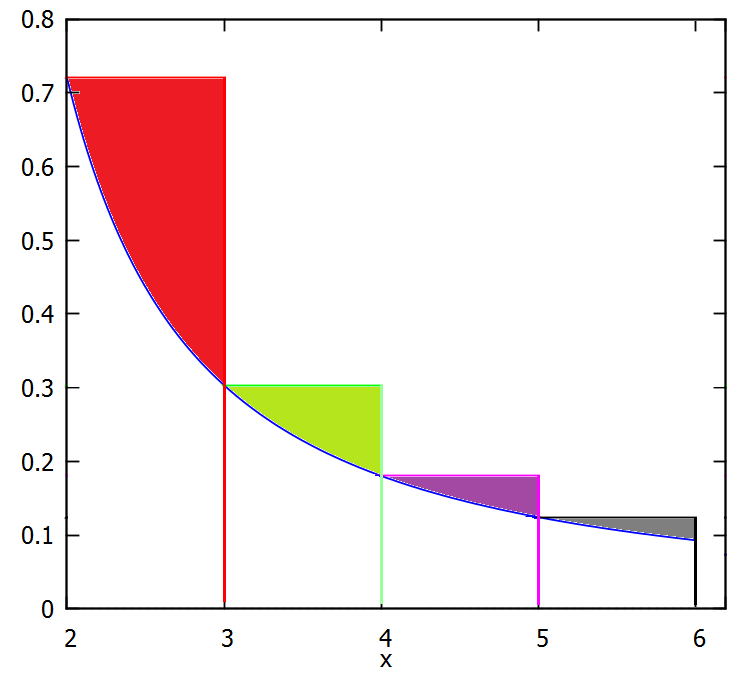
\includegraphics[width=.7\linewidth]{ExerciseI2_6_12.png}
  \caption{Plot of $1/x\log(x)$ and rectangles of height $1/n\log(n)$ and width 1.}
\label{fig:I2.6.12}
\end{figure}
%
{\bf Exercise I2.6.12}, Page 136, please see Fig.~\ref{fig:I2.6.12}. This means that
%
\nbea
\sum_{n=2}^N \frac{1}{n\log(n)} > \int_2^{N+1} \frac{1}{x\log(x)} dx
\neea
%
note the upper limit of the integral, next
%
\nbea
\int_2^{N+1} \frac{1}{x\log(x)} dx & = & \left.\log(\log(x))\right|_2^{N+1} \\
& = & \log(\log(N+1)) - \log(\log(2))
\neea
%
which goes to infinity when $N\to\infty$.

{\bf Page 143}, proof of Abel's Theorem Part I, ``Because $f_m(x)$ is just a polynomial, it is continuous. So, for some $\delta>0$, it is true that $|f_m(x) - f_m(1)|<\epsilon/3$ whenever $|x-1|<\delta$''. Recall the definition of continuity, $f(x)$ is continuous at $x=a$ if and only if
%
\nbea
\lim_{x\to a} f(x) & = & f(a)
\neea
%
and from the definition of limit, ``for every $\epsilon$ we can find a $\delta$ such that $|f(x) - f(a)|<\epsilon$ when $0 <|x-a|<\delta$''.

The next question is whether the $\delta$'s are all the same, here we have three $\delta$'s, so if they are al different we just pick the biggest one because the definition of limit/continuity only requires that for every $\epsilon$ we can find a $\delta$ and so the $\delta$ is a free variable.

\bigskip
\underline{\textit{\textbf{Chapter 6}}}
\bigskip

{\bf Page 147}, Euler's proof of the quadratic harmonic series, from Eq 6.2 we can see that we have every quadratic numbers in the denominators, $4,9,16,\ldots$ therefore we will be able to make any quartic and other even powers, but it's almost impossible to make odd powers

{\bf Page 154}, two typos, first mid of page, the substitution is reversed it should've been $x = 2iz$ instead of the other way around stated in the book, bottom of page, formula for $\cot(z)$, an overall factor of $\frac{1}{2^n}$ is missing.

\bigskip
\underline{\textit{\textbf{Chapter 8}}}
\bigskip

{\bf Exercise 8.2.1}, Page 199, first we expand
%
\nbea
1 - 2^{1-s} & = & 1 - e^{(1-s)\log(2)} \\
& = & 1 - \left ( \sum_{n=0}^\infty \frac{1}{n!} \lbrack(1-s)\log(2)\rbrack^n \right ) \\
& = & \sum_{n=1}^\infty \frac{1}{n!} (-1)^{n+1} (s-1)^n \log^n(2)
\neea
%
we now calculate the expansion for $1/(1 - 2^{1-s})$, we use long division for this, or we can use geometric series if $|s| > 1$
%
\nbea
1 & = & (1 - 2^{1-s})\times\frac{1}{(1 - 2^{1-s})} \\
& = & \left(\sum_{n=1}^\infty \frac{1}{n!} (-1)^{n+1} (s-1)^n \log^n(2)\right)\times\left(\sum_{k=-1}^\infty a_k(s-1)^k\right)
\neea
%
and so
%
\nbea
1 & = & \log(2) a_{-1} \\
0 & = & \log(2) a_0 - \frac{1}{2!}\log^2(2) a_{-1} \\
0 & = & \log(2) a_1 - \frac{1}{2!}\log^2(2) a_{0} + \frac{1}{3!}\log^3(2) a_{-1} \\
0 & = & \log(2) a_2 - \frac{1}{2!}\log^2(2) a_{1} + \frac{1}{3!}\log^3(2) a_{0} - \frac{1}{4!}\log^4(2) a_{-1}
\neea
%
and so $a_{-1} = 1/\log(2)$, $a_0 = 1/2$, $a_1 = (1/12)\log(2)$, $a_2 = 0$, $a_3 = \ldots$.

Now, as the book says that $\Phi(s) = \log(2) + O(s-1)$, since if we Taylor expand around $s=1$ we know that $\Phi(1) = \log(2)$, so the first term is indeed $\log(2)$ and since we are expanding around $s=1$ the correction terms are of order $O(s-1)$ (note that here $O(s-1)$ is bigger than $O((s-1)^m)$ since $s\to1$). Now from the definition
%
\nbea
\zeta(s) & = & \frac{1}{1-2^{1-s}} \Phi(s) \\
& = & \left( \frac{1}{\log(2)}\frac{1}{s-1} + \frac{1}{2} + \frac{\log(2)}{12}(s-1) + \ldots \right)\left( \log(2) + O(s-1)\right) \\
& = & \frac{1}{s-1} + O(1)
\neea
%
again recall here we are interested in $s\to1$ and so $O(1)$ is the biggest error, all other Big Oh are in $O((s-1)^m),~m \ge 1$

{\bf Exercise8.2.2}, Page 202, let's apply Euler operators using Maxima, so
%
\nbea
x\frac{d}{dx}\frac{-x}{(1+x)^2} & = & x\frac{d}{dx}\sum_{n=1}^\infty (-1)^n n x^n \\
\frac{x(x-1)}{(x+1)^3} & = & \sum_{n=0}^\infty (-1)^{n} {n}^2 x^{n}
\neea
%
and so $\Phi(-2) = 0$ and therefore $\zeta(-2)=0$, continuing $\mathcal{E}$
%
\nbea
\mathcal{E}^2\left(\frac{-x}{(1+x)^2}\right) & = & -\frac{x(x^2-4x+1)}{(x+1)^4} \\
\mathcal{E}^3\left(\frac{-x}{(1+x)^2}\right) & = & \frac{x(x^3-11x^2+11x-1)}{(x+1)^5} \\
\mathcal{E}^4\left(\frac{-x}{(1+x)^2}\right) & = & -\frac{x(x^4-26x^3+66x^2-26x+1)}{(x+1)^6} \\
\mathcal{E}^5\left(\frac{-x}{(1+x)^2}\right) & = & \frac{x(x^5-57x^4+302x^3-302x^2+57x-1)}{(x+1)^7} \\
\mathcal{E}^6\left(\frac{-x}{(1+x)^2}\right) & = & -\frac{x(x^6-120x^5+1191x^4-2416x^3+1191x^2-120x+1)}{(x+1)^8}
\neea
%
and the $\Phi(s)$'s are $-1$ times the above and so and connecting it to the next exercise
%
\nbea
\begin{array}{r c l c c c l}
\zeta(-1) & = & (1-2^2)^{-1}\Phi(-1) & = & -\frac{1}{12} & = & -\frac{1}{2} \times \frac{1}{6}\\
\zeta(-2) & = & (1-2^3)^{-1}\Phi(-2) & = & 0 \\
\zeta(-3) & = & (1-2^4)^{-1}\Phi(-3) & = & \frac{1}{120}  & = & -\frac{1}{4} \times -\frac{1}{30}\\
\zeta(-4) & = & (1-2^5)^{-1}\Phi(-4) & = & 0 \\
\zeta(-5) & = & (1-2^6)^{-1}\Phi(-5) & = & -\frac{1}{252} & = & -\frac{1}{6} \times \frac{1}{42}\\
\zeta(-6) & = & (1-2^7)^{-1}\Phi(-6) & = & 0 \\
\zeta(-7) & = & (1-2^8)^{-1}\Phi(-7) & = & \frac{1}{240} & = & -\frac{1}{8} \times-\frac{1}{30}
\end{array}
\neea
%

{\bf Exercise 8.2.3}, Page 203, the conjecture here is that according to the list above, $\zeta(-2n)=0$ and $\zeta(-(2n+1)) = -\frac{1}{2(n+1)}\times B_{2(n+1)}$, $n\ge0$

{\bf Exercise 8.3.2}, Page 209, Assuming $s>0$ is real, change variables by $x=t^s$ in the integral (8.4), this means $dx=st^{s-1}dt$
%
\nbea
\Gamma(s) & = & \int_0^\infty e^{-t}t^{s-1}dt \\
& = & \int_0^\infty e^{-x^{1/s}} \frac{dx}{s}
\neea
%
now change $s\to 1/s$
%
\nbea
\Gamma(1/s) & = & s \int_0^\infty e^{-x^s} dx
\neea
%
using the ``normal'' Gamma function relationship
%
\nbea
\Gamma(s+1) & = & s\Gamma(s)
\neea
%
now substituting for $s\to1/s$
%
\nbea
\Gamma(1+1/s) & = & \frac{1}{s}\Gamma(1/s) \\
& = & \frac{\cancel{s}}{\bcancel{s}} \int_0^\infty e^{-x^s} dx
\neea
%
so even for the $1/s$ Gamma, the relation is still the same
%
\nbea
\Gamma(1/s+1) & = & \frac{1}{s}\Gamma(1/s)
\neea
%
and so
%
\nbea
\Gamma(5/2) & = & \frac{3}{2} \Gamma(3/2) \\
& = & \frac{3\sqrt{\pi}}{4}
\neea
%
and $\Gamma(7/2) = 15\sqrt{\pi}/8,~\Gamma(9/2) = 105\sqrt{\pi}/16$ and so the general formula is
%
\nbea
\Gamma(n+1/2) & = & \frac{(2n-1)!!}{2^n}
\neea
%
and now
%
\nbea
\Gamma(1/2) & = & 2 \Gamma(3/2) \\
& = & \sqrt{\pi}
\neea
%
and
%
\nbea
\Gamma(-1/2) & = & -2 \Gamma(1/2) \\
& = & -2\sqrt{\pi}
\neea
%
Note that the goal of this whole exercise is to massage the Gamma function into a Gaussian integral so that we can evaluate it.

{\bf Page 211}, Eq (8.7), there's a typo, it should have been $s=-(2k-1)$, it's for negative odd integers that we have simple poles

{\bf Exercise 8.4.1}, Page 212, What are the singular parts for the Laurent expansions of $\Gamma(s)$, here we can use (8.5)
%
\nbea
\Gamma(s) & = & \sum_{k=0}^\infty \frac{(-1)^k}{k!} \frac{1}{s+k} + \int_1^\infty e^{-t}t^{s-1}dt
\neea
%
so near $s=-2n+1$ we have
%
\nbea
\Gamma(s) & = & \frac{(-1)^{2n-1}}{(2n-1)!} \frac{1}{(s+(2n-1))} + O((s+(2n-1)))
\neea
%
and so
%
\nbea
\Gamma(s)^{-1} & = & \frac{(2n-1)!}{(-1)^{2n-1}} (s+(2n-1)) + O((s+(2n-1))^2)
\neea
%
and around $s=-2n+1$
%
\nbea
F(s) + G(s) & = & \frac{B_{2n}}{(2n)!}\frac{1}{(s + (2n-1))} + O(1)
\neea
%
and so
%
\nbea
\zeta(-2n+1) & = & \Gamma(s)^{-1} \lbrack F(s) + G(s)\rbrack\\
& = & \left(\frac{(2n-1)!}{(-1)^{2n-1}} (s+(2n-1)) + O((s+(2n-1))^2)\right) \left\lbrack  \frac{B_{2n}}{(2n)!}\frac{1}{(s + (2n-1))} + O(1) \right\rbrack \\
& = & \frac{(-1)^{2n-1}B_{2n}}{2n} + O(1) \\
& = & -\frac{B_{2n}}{2n} + O(1)
\neea
%

{\bf Page 213}, lower half of the page, the formula for $\zeta(2n)$ is given in Chapter 6, Page 154 from the expansion of $z\cot(z)$

\bigskip
\underline{\textit{\textbf{Chapter 10}}}
\bigskip

{\bf Page 234}, Theorem of Eq (10.5), the {\it proof} of this theorem is actually not a proof, more like a validation check, what it actually does is that first, it shows that the Mellin transform of $\Psi(x)$
%
\nbea
-s\mathcal{M}\Psi(s) & = & \frac{\zeta'(s)}{\zeta(s)}
\neea
%
and then we show the Mellin transform of each term in $\Psi(s)$ to correspond to the terms in $\frac{\zeta'(s)}{\zeta(s)}$, but it did not show how $\Psi(x)$ was derived in the first place.

{\bf Page 236}, last sentence, this is related to Eq (10.5), we know that $\Psi(x)$ is real and so
%
\nbea
\overline{\Psi(x)} & = & \Psi(x) \\
\to \sum_\rho \frac{x^{\overline\rho}}{\overline\rho} & = & \sum_\rho \frac{x^{\rho}}{\rho}
\neea
%
and therefore the zeros $\rho$ must come in pairs of $\rho$ and $\overline\rho$

{\bf Page 244 to Page 247}, proof of Theorem, Eq (10.11), again this proof doesn't show how Riemann derived the explicit formula for $\Pi(x)$, it only shows that it is consistent by showing the relationship on Page 246
%
\nbea
\mathcal{E}\Psi(x) = \Pi(x) + \mathcal{E}(\Pi(x)\cdot\log(x))
\neea
%
since we know the explicit formula for $\Psi(x)$, the first and crucial step is of course showing
%
\nbea
\log(\zeta(s)) = s\mathcal{M}\Pi(s)
\neea
%
of Eq (10.12)

So to summarize, we have two explicit formulae, one from Von Mangoldt and one from Riemann, but the main formula is of course Riemann's explicit formula for $\Pi(x)$ and $\pi(x)$, so here's how everything is connected to the zeta function
\bit
\item First, we show that the zeta function can be represented as the Hadamard's Product
\item Next, we show that the log derivative of the conventional zeta function is just a sum of Von Mangoldt's functions, $\Psi(x)$
\item Using this equality we now substitute the Hadamard's product for the conventional zeta function and show that Von Mangoldt's function $\Psi(x)$ can be explicitly formulated by taking the ``inverse'' Mellin transform of the log derivative of Hadamard's product and this is how the Von Mangoldt's function $\Psi(x)$ is related to the zeros of the zeta function
\item With all this set, we now relate the Von Mangoldt's function to the Riemann prime counting function $\Pi(x) = \sum_k \frac{1}{k}\pi(x^{1/k})$, the relationship is quite complicated $\mathcal{E}\Psi(x) = \Pi(x) + \mathcal{E}(\Pi(x)\cdot\log(x))$
\item And this is how the Riemann prime counting function is related to the zeros of the zeta function, and using the generalized Mobius inversion we get $\pi(x)$ as a sum of $\Pi(x)$ and now we can express the original prime counting function $\pi(x)$ in terms of the zeros of the zeta function
\eit

{\bf Exercise 10.4.1}, Page 246, for $\alpha=1, \rho,$ or $2n$, show that
%
\nbea
x\frac{d}{dx}\left(\frac{x^\alpha}{\alpha}\right) = -{\rm Li}(x^\alpha) +x\frac{d}{dx} ({\rm Li}(x^\alpha)\cdot\log(x))
\neea
%
I think it's easier to start with the second term of the RHS
%
\nbea
x\frac{d}{dx} ({\rm Li}(x^\alpha)\cdot\log(x)) & = & x \log(x) \frac{d}{dx} {\rm Li}(x^\alpha) + x{\rm Li}(x^\alpha)\frac{d}{dx} \log(x) \\
& = & x\log(x)\frac{d}{dx}\left(\int_0^{x^\alpha}\frac{dt}{\log(t)}\right) + x{\rm Li}(x^\alpha)\frac{1}{x} \\
& = & x\log(x) \frac{1}{\log(x^\alpha)}\cdot\frac{d}{dx}(x^\alpha) + {\rm Li}(x^\alpha) \\
& = & \frac{\bcancel{\alpha \log(x)}~~ x^\alpha}{\bcancel{\log(x^\alpha)}} + {\rm Li}(x^\alpha) \\
& = & x^\alpha + {\rm Li}(x^\alpha)
\neea
%

{\bf Page 248}, top of page, on inverting $\Pi(x)$, this is almost the same strategy as the one used for Euler's product of the zeta function, first
%
\nbea
\frac{1}{2} \Pi(x^{1/2}) & = & \frac{1}{2}\pi(x^{1/2}) + \frac{1}{4}\pi(x^{1/4}) + \frac{1}{6}\pi(x^{1/6}) + \ldots
\neea
%
subtracting this from $\Pi(x)$
%
\nbea
\Pi(x) - \frac{1}{2} \Pi(x^{1/2}) & = & \left (\pi(x) + \cancel{\frac{1}{2}\pi(x^{1/2})} + \frac{1}{3}\pi(x^{1/3}) + \ldots + \cancel{\frac{1}{6}\pi(x^{1/6})} + \ldots \right) - \\
&& ~~~~~~~~~\left ( \cancel{\frac{1}{2}\pi(x^{1/2})} + \frac{1}{4}\pi(x^{1/4}) + \cancel{\frac{1}{6}\pi(x^{1/6})} + \ldots\right )
\neea
%
removes any term $\frac{1}{k}\pi(x^{1/k})$ with $k$ a multiple of two, so we kind of see the pattern, we need to keep subtracting $\Pi(x^{1/p})$ where $p$ is prime, but, as the example above shows, $\frac{1}{6}\pi(x^{1/6})$ is already removed by $-\Pi(x^{1/2})$, subtracting $\Pi(x^{1/3})$ will doubly remove $\frac{1}{6}\pi(x^{1/6})$, therefore we need to add this back and note that the first term of $\Pi(x)$, \ie $\pi(x)$ is never removed with these subtractions
%
\nbea
\pi(x) & = & \Pi(x) - \frac{1}{2}\Pi(x^{1/2}) - \frac{1}{3}\Pi(x^{1/3}) + \frac{1}{6}\Pi(x^{1/6}) + \ldots
\neea
%
but it's a bit hard to keep track these subtractions and addition, but this is how we get the inversion. An easier (and more historically accurate) way is to use the generalized Mobius inversion formula as follows
%
\nbea
G(x) = \sum_{n=1}^\infty \frac{1}{n} F(x^{1/n}) &~~~~~\longleftrightarrow~~~~~& F(x) = \sum_{n=1}^\infty \frac{\mu(n)}{n} G(x^{1/n})
\neea
%
but how do we see that this is correct, the easiest way is back substitution
%
\nbea
G(x) & = & \sum_{n=1}^\infty \frac{1}{n} F(x^{1/n}) \\
& = & \sum_{n=1}^\infty \frac{1}{n} \left(\sum_{m=1}^\infty \frac{\mu(m)}{m} G\left(\left(x^{1/n}\right)^{1/m}\right)\right) \\
& = & \sum_{n=1}^\infty\sum_{m=1}^\infty \frac{\mu(m)}{mn} G\left(x^{1/(nm)}\right)
\neea
%
we now rearrange the sum as follow, group all $G\left(x^{1/(nm)}\right)$ with the same $mn=c$ and so
%
\nbea
\sum_{n=1}^\infty\sum_{m=1}^\infty \frac{\mu(m)}{mn} G\left(x^{1/(nm)}\right) & = & \sum_{c=1}^\infty G\left(x^{1/c}\right) \sum_{d|c} \frac{\mu(d)}{d\left(\frac{c}{d}\right)} \\
& = & \sum_{c=1}^\infty G\left(x^{1/c}\right) \sum_{d|c} \frac{\mu(d)}{c} \\
& = & \sum_{c=1}^\infty G\left(x^{1/c}\right) \frac{1}{c} \sum_{d|c} \mu(d) \\
& = & \sum_{c=1}^\infty G\left(x^{1/c}\right) \frac{1}{c} \delta_{c,1} \\
& = & G(x)
\neea
%
so it works, the only thing left to fill is that why $\sum_{d|c} \mu(d) = \delta_{c,1}$ where $\delta_{c,1}$ is kronecker delta, there's a proof of this in a direct way in Apostol but let's not do it that way, let start with the Euler's product
%
\nbea
\sum_{n=1}^\infty \frac{1}{n} & = & \prod_p \left(1 - \frac{1}{p}\right)^{-1}
\neea
%
taking $s=1$ in the zeta function, taking the reciprocal
%
\nbea
\frac{1}{\sum_{n=1}^\infty \frac{1}{n}} & = & \prod_p \left(1 - \frac{1}{p}\right) \\
& = & \left(1 - \frac{1}{2}\right)\left(1 - \frac{1}{3}\right)\left(1 - \frac{1}{5}\right)\ldots \\
& = & \sum_{n=1}^\infty \frac{\mu(n)}{n}
\neea
%
because each $\frac{1}{p}$ carries a minus sign in front of it, and there's only one factor for each prime so there won't be anything of the form $\frac{1}{3^2}$ or $\frac{1}{5^9}$, \ie anything with duplicate primes. And since the initial product is over all primes we cover all $n$ with distinct primes and so the $\sum_{n=1}^\infty$ in the last line and also for a single prime the sign is always minus and for an odd number of prime as well and for an even number of primes the sign will be positive, this is the definition of $\mu(n)$. More generally
%
\nbea
\zeta(s) = \sum_{n=1}^\infty \frac{1}{n^s} &~~~~~\longleftrightarrow~~~~~& \frac{1}{\zeta(s)} = \sum_{n=1}^\infty \frac{\mu(n)}{n^s}
\neea
%
the proof of which is exactly the same for the case of $s=1$.

So what does it have to do with $\sum_{d|c} \mu(d) = \delta_{c,1}$? well, let's multiply them
%
\nbea
\left(\prod_p \left(1 - \frac{1}{p^s}\right)^{-1}\right) \left(\prod_p \left(1 - \frac{1}{p^s}\right) \right) & = & \sum_{n=1}^\infty \frac{1}{n^s}\sum_{m=1}^\infty \frac{\mu(m)}{m^s}\\
1 & = & \sum_{n=1}^\infty\sum_{m=1}^\infty \frac{\mu(m)}{(mn)^s} \\
\sum_{c=1}\frac{a_n}{c^s} & = & \sum_{c=1}^\infty\sum_{d|c} \frac{\mu(d)}{c^s} \\
\sum_{c=1}\frac{a_n}{c^s} & = & \sum_{c=1}^\infty \frac{\left(\sum_{d|c}\mu(d)\right)}{c^s}
\neea
%
where $a_n = 1$ where $n=1$ and $a_n=0$ otherwise, we now only need to compare the coefficient for each $1/c^s$ and in this case it's very easy
%
\nbea
a_1 & = & \sum_{d|1}\mu(d) \\
\to 1 & = & \mu(1)
\neea
%
which is consistent and for all other $a_{n>1} = 0 = \sum_{d|c>1}\mu(d) = 0$ which means that $\sum_{d|c}\mu(d) = \delta_{c,1}$


{\bf Page 248}, middle of page, ``a consequence of Prime Number Theorem says that $\sum_n \mu(n)/n=0$'', this result can be obtained without the prime number theorem, it is in fact a very clever trick by Mobius as follows.

With the above trick Mobius showed that $\sum_{n=1}^\infty \frac{\mu(n)}{n} = 0$, here's how. First, just like above the following relationship is also true
%
\nbea
G(x) = \sum_{n=1}^\infty a_n F(x) &~~~~~\longleftrightarrow~~~~~& F(x) = \sum_{n=1} b_n G(x)
\neea
%
express $G(x)$, $F(x)$ in terms of power series
%
\nbea
\sum_{j=0}^\infty g_j x^j & = & \sum_{n=1}^\infty a_n \left(\sum_{m=1}^\infty b_m \left(\sum_{i=0}^\infty g_i x^i\right)\right) \\
& = &\sum_{i=0}^\infty \left( \sum_{n=1}^\infty\sum_{m=1}^\infty a_n  b_m \right) g_i x^i \\
& = &\sum_{i=0}^\infty \left( \sum_{c=1}^\infty\sum_{d|c} a_{\frac{c}{d}}  b_{d} \right) g_i x^i
\neea
%
again comparing coefficients of same power of $x$ on both sides we get that
%
\nbea
1 = \sum_{c=1}^\infty\sum_{d|c} a_{\frac{c}{d}}  b_{d} & = & \sum_{c=1}^\infty\sum_{d|c} a_c  b_{\frac{c}{d}} \\
\to \sum_{d|c} a_c  b_{\frac{c}{d}} & = & \delta_{c,1}
\neea
%
this can be immediately generalized into
%
\nbea
G(x) = \sum_{n=1}^\infty a_n F(x^n) &~~~~~\longleftrightarrow~~~~~& F(x) = \sum_{n=1}^\infty b_n G(x^n)
\neea
%
because by the same token as before (but not expanding each function into power series)
%
\nbea
G(x) & = & \sum_{n=1}^\infty a_n \left(\sum_{m=1}^\infty b_m G\left (\left(x^n\right)^m\right)\right) \\
& = & \sum_{n=1}^\infty \sum_{m=1}^\infty a_n b_m G(x^{nm}) \\
& = & \sum_{c=1}^\infty G(x^c) \sum_{d|c} a_{d} b_{\frac{c}{d}} \\
\to \sum_{d|c} a_{d} b_{\frac{c}{d}} & = & \delta_{c,1}
\neea
%
with the same conclusion (and again we are rearranging the double sum into a sum for a fixed exponent for $x$ and a sum for the factors of $c$). This is more or less the generalization of our previous case involving $\Pi(x)$ and $\pi(x)$, note that since $\sum_{c|d}$ involves all factors of $c$ so we can swap $a_{\frac{c}{d}}  b_{d} ~\leftrightarrow~ a_d  b_{\frac{c}{d}}$ inside the sum $\sum_{d|c}$. The series $\sum_{n=0}^\infty \frac{f_n}{n^s}$ is normally called Dirichlet series in the literature.

Mobius then cleverly applied this good finding on our beloved geometric series by setting $a_n=1$ and $b_n=\mu(n)$ for all $n$
%
\nbea
\frac{x}{1-x} = \sum_{n=1}^\infty x^n &~~~~~\longleftrightarrow~~~~~& x = \sum_{n=1}^\infty \mu(n) \frac{x^n}{1-x^n}
\neea
%
again since as shown above that $\sum_{d|c}\mu(d) = \delta_{c,1}$. He then noticed that if $x\to1$ we have $1-x = \epsilon$ and
%
\nbea
1-x^n & = & 1- (1-\epsilon)^n \\
& = & 1 - ( 1 - n\epsilon + O(\epsilon^2) ) \\
& = & n\epsilon + O(\epsilon^2)
\neea
%
where we just expanded $(1-\epsilon)^n$ using the binomial theorem, therefore
%
\nbea
\frac{x^n}{1-x^n} & = & \frac{1 + O(\epsilon)}{n\epsilon + O(\epsilon^2)} \\
& = & \frac{1}{n\epsilon}(1+O(\epsilon))\left(\frac{1}{1 + O(\epsilon)}\right) \\
& = & \frac{1}{n\epsilon}(1+O(\epsilon))\left(1 + O(\epsilon)\right) \\
& = & \frac{1}{n\epsilon}+O(1)
\neea
%
therefore
%
\nbea
x & = & \sum_{n=1}^\infty \mu(n) \frac{x^n}{1-x^n} \\
1 + \epsilon & = & \sum_{n=1}^\infty \mu(n) \left(\frac{1}{n\epsilon}+O(1) \right)
\neea
%
multiplying both sides by $\epsilon$
%
\nbea
\epsilon + \epsilon^2 & = & \sum_{n=1}^\infty \frac{\mu(n)}{n}+O\left(\epsilon\sum_{n=1}^\infty \frac{\mu(n)}{n}\right)
\neea
%
the thing to note here is that the above is true for any $\epsilon$, this means that $\sum_{n=1}^\infty \frac{\mu(n)}{n}$ is finite, but if it's finite since $\epsilon\to0$ the only choice is $\sum_{n=1}^\infty \frac{\mu(n)}{n} = 0$

{\bf Page 249 and Page 250}, proof of Theorem, Eq (10.15), to get the last line on Page 249
%
\nbea
\re\{\log(z)\} & = & \re \{\log(r e^{i\theta})\} \\
& = & \re\{\log(r) + i(\theta + 2\pi n)\} \\
& = & \re\{\log(r)\} \\
& = & \re\{\log(|z|)\} \\
& = & \log(|z|)
\neea
%
the actual kick here is on Page 250, where ``suppose that $t$ is $\ldots$ a zero of the form $1+i\gamma$'' and it leads to a contradiction so this covers the case for $\re(\rho) = 1$, how about the other boundary $\re(\rho) = 0$, since we have shown that there's no zero with $\re(\rho) = 1$, by symmetry, $\Lambda(1-s) = \Lambda(s)$, there is no zero with $\re(\rho)=0$ either.

Also, here $\epsilon\to0$ from $> 1$, the other thing is that we try to take the limit $\epsilon\to1$ from below the argument for the Big Oh still works so we will still have a contradiction except for the fact that $\zeta(s)$ is only defined for $\re(s) > 1$ so the limit must be taken from above

\bigskip
\underline{\textit{\textbf{Interlude 4}}}
\bigskip

{\bf Page 258}, Hensel's Lemma, this is my alternative proof, also I found the statement that $x_{j+1}$ to be unique is not quite right, even for the example of $a=-1$ and $p=5$, $x_1=2$, I can get $x_2 = 32$ and $32^2 = 1024 = -1 + 25\cdot 41$, in his example his $x_2 = 7$ with $7^2 = 49 = -1 + 25\cdot 2$ so I believe what he meant by unique is that it is unique modulo $p^{j+1}$.

Now here is my proof, say there's a solution to $x_j^2 \equiv a \pmod{p^j}$, if there's another solution at all, it must be of the form
%
\nbea
x_{j+1} & = & x_j + mp^j \\
\to x_{j+1}^2 & = & (x_j + mp^j)^2 \\
& = & x^2_j + 2x_jmp^j + m^2p^{2j} \\
& = & (a + np^j) + 2x_jmp^j + m^2p^{2j}
\neea
%
for the RHS to be $a \pmod{p^{j+1}}$, $n+ 2x_jm$ must be a multiple of $p$ and this is actually guaranteed by Bezout's lemma, here's how. What we need is
%
\nbea
n+ 2x_jm & = & pw
\neea
%
if $\gcd(2x_j,p)=1$ then we are done since Bezout guarantee that there would be an $m'$ and a $w'$ such that
%
\nbea
1 & = & (2x_j)m' + pw'
\neea
%
multiplying both sides by $n$ we get our solution, but what if $\gcd(2x_j,p) = d > 1$? since $p$ is prime, the only possible values for $d$ is $d=p=2$ or $d = p$, first let's take $d = p \neq 2$, this means that $p|x_j$ since $p\nmid 2$
%
\nbea
x_j^2 & = & a +p^jn \\
p(p{x'}_j^2) & = & a +p(p^{j-1}n)
\neea
%
but this means that $a \equiv 0 \pmod{p}$, which is not allowed by the assumption of the lemma, \ie $a \not\equiv 0 \pmod{p}$ right at the beginning of the lemma, so the only other alternative is $d = p = 2$, but this case is excluded because the lemma only concerns odd $p$ :) but why won't $p=2$ work? if you look back at our crucial equation
%
\nbea
n+ 2x_jm & = & 2w
\neea
%
this means that $n$ has to be even and so it's not guaranteed that as long as $x_j^2 \equiv a \pmod{2^j}$ we'll have another solution $x_{j+1}^2 \equiv a \pmod{2^{j+1}}$, only on certain cases this will hold, but the case for odd $p$ will {\it always} hold.

Coming back to uniqueness modulo $p^{j+1}$, from Bezout's lemma we know that if $\gcd(a,b)=d$ there exist $x,y$ such that $ax+by=d$, it so happens that these $x,y$ are not unique, any other
%
\nbea
x' = x + c\cdot\frac{b}{d} & ~~~~~~~~~ & y' = y - c\cdot\frac{a}{d}
\neea
%
also work where $c$ is any integer. Applying it to our case, what we have is
%
\nbea
1 & = & 2x_j(-m') + pw' \\
\to n & = & 2x_j(-m) + pw
\neea
%
and so any $-M' = -m' - c\cdot p \to -M = (-m - ncp)$ is also a solution for any integer $c$, note that this $M$ plays its role in
%
\nbea
x_{j+1} & = & x_j + Mp^j \\
& = & x_j + mp^j + ncp^{j+1}
\neea
%
and so it differs from another $x_{j+1}$ by a multiple of $p^{j+1}$

\bigskip
\underline{\textbf{\textit{Chapter 11}}}
\bigskip


\bigskip
\underline{\textbf{\textit{Chapter 12}}}
\bigskip

{\bf Page 284}, just a fun note:) So it is always possible to turn a cubic equation into an elliptical curve 
%
\nbea
y^2 = x^3 - 432D^2 & ~~~~~ \longleftrightarrow ~~~~~& X^3 + Y^3 = D
\neea
%
with the following transformation (note that in the above everything is rational)
%
\nbea
X = \frac{36D+y}{6x}~, &~~~~~~~~~~& Y = \frac{36D-y}{6x} \\
x = \frac{12D}{X+Y}~, &~~~~~~~~~~& y = 36D~\frac{X-Y}{X+Y}
\neea
%
and this is how Fermat's Last Theorem is connected to elliptical curves, see also Page 285 on this relationship used by Andre Wiles.

{\bf Page 288}, after Eq (12.3), ``there are $1 + \left(\frac{f(x)}{p}\right)$'', note that it is not a division, that is the Legendre symbol, and it makes sense, if $f(x)$ is a quadratic residue then there are two roots for $y$ and therefore there are $1+1=2$ roots, if $f(x)$ is {\bf not} a quadratic residue then there are no roots, \ie $1-1=0$ root, and if $f(x) \equiv 0 \pmod{p}$ there there's only, $1+0=1$ root for $y$ which is $y=0$.

{\bf Page 289}, Theorem Eq (12.4), if you forget what $a(p)$ is, it is defined on Page 287, $a(p) = p+1-N_p$

{\bf Page 291}, lower half of page, ``The discriminant $\ldots$ $\Delta=-16(4A^3 + 27B^2)$; for the finitely many primes $p$ dividing $\Delta$, the Euler factor at $p$ has a different definition.'' This is because $p|\Delta$ means that $\Delta \equiv 0 \pmod{p}$, zero discriminant means we have singular points on the curve, either a crossing or a kink, so that's why the meaning is different :)

\bigskip
\underline{\textit{\textbf{Chapter 13}}}
\bigskip

{\bf Page 295}. These theorems are easy to prove in one direction but hard in the other, if there are $x,y$ such that $x^2 + y^2 = p$ then
%
\nbea
x^2 + y^2 & = & p \\
\to x^2 + y^2 & \equiv & 0 \pmod{p} \\
x^2 & \equiv & -y^2 \pmod{p} \\
\left(\frac{x^2}{y^2}\right) & \equiv & -1 \pmod{p}
\neea
%
and so $-1$ is a quadratic residue modulo $p$, this means that
%
\nbea
(-1)^{\frac{p-1}{2}} & = & +1 \\
\to p & = & 4n + 1
\neea
%
but proving that there are $x^2,y^2 < p$ such that $x^2+y^2=p$ given that $p = 4n+1$ is difficult, the thing is that even if we show that $-1$ is a quadratic residue, the only thing we are saying is that we can find $x^2 + y^2 = pn$ but $n$ is not necessarily 1 (we can get this by reversing the process above regarding $-1$ modulo $p$). The same tactic can be used $x^2 + |N|y^2 = p$. The proof of the converse for $p\equiv 1 \pmod{4} \Rightarrow x^2+y^2 = p$ can be found on Stein's ent.pdf on the chapter of continued fraction, his proof is really cool, another popular proof is by Euler but it's quite tedious.

{\bf Page 297}, upper half of page. The determinant of a product of matrices is the product of the determinants and so having determinant one preserves the group structure. If it had been $-1$ the determinants would oscillate between $+1$ and $-1$ when we do the group operation.

{\bf Page 298}, top paragraph, we are changing $(x,y)$ into $(-y,x)$ instead of $(y,x)$ because we want the determinant to be $+1$, $(y,x)$ will have determinant $-1$

{bf Page 298}, upper half of page. Note that this is \underline{\textbf{\textit{not}}} a similarity transform, it looks similar but it's not. If you take a product between a vector and a matrix say $FV$, to do a similarity transform we need to transform both the vector and the matrix, \ie
%
\nbea
M(FV) & = & M(FM^{-1}MV) \\
& = & (MFM^{-1})MV
\neea
%
because if you change the basis for the vector you need to change it for the matrix as well so if you sandwich the matrix between two vectors like what we are doing to calculate $F(x,y)$ what you get is
%
\nbea
VFV & \to & VM^{-1}(MFM^{-1})MV
\neea
%
and this is a similarity transform, it preserves the sandwich product and there are {\bf four} copies of $M$ not just two like the one in the book, let's see this with a simple example. Changing $(x,y) \to (-y,x)$ for $2x^2 + 3y^2$
%
\nbea
\left(
\begin{array}{c c}
0 & -1 \\
1 & 0
\end{array}
\right)
\left(
\begin{array}{c c}
2 & 0 \\
0 & 3
\end{array}
\right)
\left(
\begin{array}{c c}
0 & 1 \\
-1 & 0
\end{array}
\right) & = & 
\left(
\begin{array}{c c}
3 & 0 \\
0 & 2
\end{array}
\right)
\neea
%
which means that
%
\nbea
F'(x,y) & = & 3x^2 + 2y^2
\neea
%
so for the same $(x,y)$ value, \eg $(5,7)$
%
\nbea
F'(5,7) & \neq & F(5,7) \\
173 & \neq & 197
\neea
%
if this were a similarity transform $F'(5,7)$ would be equal to $F(5,7)$.

Note also that since the matrix $F$ is symmetric, it can be diagonalized using orthogonal matrices, \ie matrices that have their transpose as their inverse. But this info is not relevant to us.

{\bf Page 299}, on Proof of Theorem, What guarantee do we have that by reducing the sum $a+c$ we will not reduce $c$ into negative territory? The reason is the discriminant $d = b^2 - 4ac < 0$ and so $b^2$ cannot be bigger than $4ac$, and doing the $M$ transformations will not change the discriminant. So in this case $c$ will not become negative to maintain $d$ and $a$ stays the same after every transformation and so $4ac$ will not change sign.

But the more important question is whether $|b| \le a$ before $c$ reaches its minimum point? because by then we cannot reduce $b$ any more. The only recourse is to then reduce $b$ using the other transformation that maintains $c$ but reduces $b$ and $a$, but we have the same question, will we reach the minimum of $a$ before reaching $b \le a \le c$? ~ \dunno

{\bf Page 299}, bottom of page, ``$b^2\equiv d \pmod{4}$ and, thus, $b\equiv d\mod2$'', this is because the only quadratic residue modulo 4 is $0$ and $1$, if $b^2 \equiv 0 \pmod{4}$ then
%
\nbea
b^2 & = & 4n \\
b & = & 2m \\
\to b & \equiv & 0 \pmod{2}
\neea
%
and the same goes if $b^2\equiv 1 \pmod{4} = 1  + 4n$, this means that $b$ is odd, therefore $b \equiv 1\pmod{2}$. The above statement is not true in general but modulo 4 is quite special

{\bf Page 301}, Theorem at the bottom of page, the wording is very confusing, what it is saying is that every form with discriminant $d$ is equivalent to one form satisfying $|b| \le a \le c$, the thing here is that since $b$ is in absolute value we have two choices $\pm b$, and the theorem says that $b \ge 0$, but then there's an if that confuses the whole thing.

If you see the proof you'll see that if $b=0$ or $|b|=a$ or $c=a$ then $\{a,b,c\} \sim \{a,-b,c\}$, so, if say a form is equivalent to $\{a,-|b|,c\}$, by the statement above it is also equivalent to $\{a,|b|,c\}$ as long as $b=0$ or $|b|=a$ or $c=a$. This is because if $F$ is equivalent to $G$ and $G$ is equivalent to $H$ then $F$ is equivalent to $H$. So it is equivalent to exactly one form with $b\ge 0$.

If $b\neq0$ nor $|b|\neq a$ nor $c\neq a$ then the form is still equivalent to a form except that we don't know whether $b$ is positive, negative, or zero. That's all

{\bf Page 302}, before and Eq (13.5), this is now strict inequality because now we are not considering $b\ge 0$, so we don't have the cases of $|b|=a$ or $c=a$ and so none of them are equal.

{\bf Page 302}, ``Then, $a=F'(1,0)=F(r,s)$. From (13.5) $\ldots$'', it's most likely not from (13.5) not, more likely from (13.2), the definition of $F(x,y)$, substituting $x=r, y=s$
%
\nbea
a & = & ar^2 + brs + cs^2
\neea
%
and so $r = \pm1$ and $s=0$.

{\bf Page 302}, second last paragraph, again some ambiguity, ``A form that satisfies the inequalities (13.4) is called REDUCED''. The thing here is that it only concerns the inequality not so much the ``and $b\ge0~\ldots$'', just the inequality. 

{\bf Page 303}, the inequality in the first paragraph, I believe the plus sign should have been a minus sign, because if $a=c$ then
%
\nbea
4ac = 4c^2 & = & b^2 - d \\
\to c & = & \sqrt{\frac{b^2 - d}{4}}
\neea
%

{\bf Page 303}, some remarks on the preceding theorems, they give us an algorithm to compute the number of classes but not the explicit formula for the number of classes, if you want the number of classes you need to run through the algorithm.

{\bf Exercise 13.1.10}, Page 305, show that $5$ is not represented by any form of discriminant $-23$ but that 3 is. Show that $6$ is represented more than one way, this will be an interesting exercise to do :)

First, if an integer $n$ is represented by a form with a discriminant $d$ then we can find an equivalent form $\{n,m,l\}$ where $m^2 \equiv d \pmod{4n}$ and $0\le m<2n$.

So as a necessary condition we need to find out if $m^2 \equiv d \pmod{4n}$, here $n=5$, $d=-23$ and so we need to find $m^2 \equiv -23 \pmod{4\cdot5}$, \ie $m^2 \equiv -23 \pmod{20} \equiv 17 \pmod{20}$ but sadly 17 is not a quadratic residue modulo 20, the quadratic residues are $1,4,9,16,5,0$.

For $n=6$ what we want is $m^2 \equiv -23 \pmod{4\cdot6} \equiv 1 \pmod{24}$ and 1 is obviously a quadratic residue modulo 24, the roots of 1 modulo 24 are $1, 5, 7, 11,13,17,19,23$, so those are the possible values for $m$

{\bf Page 303 and Page 305 and Page 306}, Theorem regarding representation and equivalence to $\{n,m,l\}$ and counting how many representations a form can have. So what it actually means is that the same form can contain multiple different $m$'s and hence the same class can represent different $m$'s, of course with the same $n$. What confused me initially was that I thought each $m$ must belong to its own class, but this seems to not be so and it makes sense.

Say there are two points $F(r,s) = n$ and $F(r',s') = n$, and these two points represent different $m$'s and there's nothing preventing these two points from representing different $m$'s if you follow the procedure of the Theorem, but these two points are produced by the same form $F$ and thus one form (or one class) can indeed represent two (or more) different $m$'s. And of course some form might not represent $n$ at all and in this case $r_F(n) = 0$.

{\bf Page 306}, here the factor of $\frac{1}{w}$ is more for $r_d(n)$, if we do not divide by $w$ then we will double count several points, for example, for $d < -4$, for each $m$ we have $F(r,s)$ and $F(-r,-s)$ representing the {\bf same} $m$ if we do not divide by $w=2$, when we sum $r_F(n)$ over classes to get $r_d(n)$, we will count both $F(r,s)$ and $F(-r,-s)$ but these two points represent the same $m$ and we would have double counted.

{\bf Page 307} Proof of Theorem, the application Chinese remainder theorem here is what is called the Chinese Remainder Map in Shoup's number theory book, basically
%
\nbea
m & \equiv & (m_{11},m_{12}) \pmod{p_1^{j_1}} \\
 & \vdots & \\
m & \equiv & (m_{k1},m_{k2}) \pmod{p_k^{j_k}}
\neea
%
note that $d \equiv m^2$ is fixed as it is the discriminant (and these different values of $m$'s give the same value of $m^2$), so basically you have some kind of a binary map
%
\nbea
m \equiv d & \equiv & (m_1, m_2, \ldots, m_k)
\neea
%
where each $m_i$ can take the value of either $m_{i1}$ or $m_{i2}$ modulo $p_i^{j_i}$, since there are only two choices for each bin and there are $k$ bins, there are therefore $2^k$ combinations. Note that the $m$ modulo $q$'s are fixed since there is only one solution for each $q$ so they do not change the number of combinations.

This is a powerful way of looking at things since this Chinese Remainder Map is unique for each number, see Shoup's book for details.

{\bf Page 307}, Proof of Theorem, the statement ``'' is there to set the base case for Hensel's lemma. Because if we have two solutions for $p$ then we again have two solutions for $p^2$ and of course another two for $p^3$ and so on, recall that Hensel's lemma only applies once you have a base case, you can't just claim that there are two solutions $x^2$ for some modulo $p^{j+1}$

{\bf Page 308}, bottom of page, the definition of $\left(\frac{d}{2}\right)$, the funny thing is that what happens when $d \equiv 3,7 \pmod{8}$? $0,2,4,6 \pmod{8}$ are all even so they're covered by the first case but from the proof of Lemma on Page 309, $\left(\frac{d}{2}\right) = \left(\frac{2}{|d|}\right)$ with $d$ odd we can see the pattern is more like
%
\nbea
\left(\frac{d}{2}\right) & = & (-1)^{(d^2-1)/8}
\neea
%
because
%
\nbea
((1 \pmod{8})^2 - 1)/8 & = & (1^2 + 2\cdot1\cdot8m + 8^2m^2 - 1)/8 \\
& = & 2m + 8m^2 \\
\to (-1)^{2m + 8m^2} & = & +1 \\
((5 \pmod{8})^2 - 1)/8 & = & (25^2 + 2\cdot5\cdot8m + 8^2m^2 - 1)/8 \\
& = & 3 + 10m + 8m^2 \\
\to (-1)^{3 + 10m + 8m^2} & = & -1
\neea
%
and so, doing the same thing for $3,7 \pmod{8}$ we get
%
\nbea
((3 \pmod{8})^2 - 1)/8 & = & (3^2 + 2\cdot3\cdot8m + 8^2m^2 - 1)/8 \\
& = & 1 + 6m + 8m^2 \\
\to (-1)^{1 + 6m + 8m^2} & = & -1 \\
((7\pmod{8})^2 - 1)/8 & = & (7^2 + 2\cdot7\cdot8m + 8^2m^2 - 1)/8 \\
& = & 6 + 14m + 8m^2 \\
\to (-1)^{6 + 14m + 8m^2} & = & +1
\neea
%
so I think the full rule is
%
\nbea
\left(\frac{d}{2}\right) & = &
\left \{
\begin{array}{l c l}
0, & ~~~ & {\rm~if~} 2|d,\\
+1, & ~~~ & {\rm~if~} d \equiv 1,7 \pmod{8},\\
-1, & ~~~ & {\rm~if~} d \equiv 3,5 \pmod{8}.
\end{array}
\right.
\neea
%

{\bf Page 310}, upper half of page, typo on the definition of $L(s,\chi_d)$, it should have been
%
\nbea
L(s,\chi_d) & = & \sum_{n=1}^\infty \chi_d(n) n^{-s}
\neea
%

{\bf Page 311}, definition of $\zeta(s,F)$, there's an apostrophe on the sum, this is because we are only summing over $(x,y) \neq (0,0)$.

{\bf Page 312}, bottom half of page, ``Thin Air Equation'' LOL I also wonder about these thin air equations as to how the heck people came up with these ``Let $x=\ldots$ and then somehow it miraculously solved the problem''

{\bf Page 312}, Lemma (Thin Air Equation, Part I), to get to the last line, let's process it term by term
%
\nbea
\sum_{k=0}^\infty \chi_d(p)^k p^{-ks} & = & \chi_d(p)^0 p^{-0\cdot s} + \chi_d(p)^1 p^{-1\cdot s} + \sum_{k=2}^\infty \chi_d(p)^k p^{-ks} \\
& = & 1 + \chi_d(p) p^{-s} + \sum_{k=2}^\infty \chi_d(p)^k p^{-ks}
\neea
%
the second term on the RHS is
%
\nbea
\sum_{k=0}^\infty \chi_d(p)^k p^{-(k+1)s} & = & \sum_{k=1}^\infty \chi_d(p)^{k-1} p^{-ks} \\
& = & \chi_d(p)^{1-1} p^{-1\cdot s} + \sum_{k=2}^\infty \chi_d(p)^{k-1} p^{-ks} \\
& = & p^{-s} + \sum_{k=2}^\infty \chi_d(p)^{k-1} p^{-ks}
\neea
%
and so combining the two
%
\nbea
\sum_{k=0}^\infty \chi_d(p)^k p^{-ks} + \sum_{k=0}^\infty \chi_d(p)^k p^{-(k+1)s} & = & \left(1 + \chi_d(p) p^{-s} + \sum_{k=2}^\infty \chi_d(p)^k p^{-ks}\right) + \left(p^{-s} + \sum_{k=2}^\infty \chi_d(p)^{k-1} p^{-ks} \right) \\
& = & 1 + (1 + \chi_d(p))p^{-s} + \sum_{k=2}^\infty (\chi_d(p)^{k-1} + \chi_d(p)^k)p^{-ks}
\neea
%

{\bf Page 313}, top of page, ``If we now multiply all the Euler factors together, the coefficient of $n^{-s}$ is $r_d(n)$, according to (13.7)''. First, the equation above the aforementioned sentence, if $\chi_d(p) = 1$ we have
%
\nbea
1 + (1 + 1)p^{-s} + \sum_{k=2}^\infty (1 + 1)p^{-ks} & = & 1 + 2\sum_{k=1}^\infty p^{-ks}
\neea
%
so the sum over $k$ starts with $k=1$. Next, note that 
%
\nbea
\chi_d(p) & = & \left(\frac{d}{p}\right)
\neea
%
and Eq (13.7) is
%
\nbea
r_d(n) & = & \left \{
\begin{array}{l c l}
0, & ~~~ & {\rm if~} p^2|n {\rm ~for~some~} p|d, \\
\prod_{\substack{p|n\\ (p,d)=1}} \left\{1 + \left(\frac{d}{p}\right)\right\}, & ~~~ & {\rm otherwise}.
\end{array}
\right.
\neea
%
Now let's say that $n = p_1^{j_1}p_2^{j_2}p_3^{j_3}p_4$ and $p_1|d$, $p_2\nmid d$, $p_3\nmid d$ and $p_4|d$ and also
%
\nbea
\chi_d(p_1) & = & \left (\frac{d}{p_1}\right) = 0 \\
\chi_d(p_2) & = & \left (\frac{d}{p_2}\right) = +1 \\
\chi_d(p_3) & = & \left (\frac{d}{p_3}\right) = -1 \\
\chi_d(p_4) & = & \left (\frac{d}{p_4}\right) = 0
\neea
%
the above is to cover all of the cases in Eq (13.7), therefore
%
\nbea
\frac{1 + p_1^{-s}}{1-\chi_d(p_1)p_1^{-s}} & = & 1 + p_1^{-s} \\
\frac{1 + p_2^{-s}}{1-\chi_d(p_2)p_2^{-s}} & = & 1 + 2\sum_{k=1}^\infty p_2^{-ks} \\
\frac{1 + p_3^{-s}}{1-\chi_d(p_3)p_3^{-s}} & = & 1 \\
\frac{1 + p_4^{-s}}{1-\chi_d(p_4)p_4^{-s}} & = & 1 + p_4^{-s}
\neea
%
combining everything
%
\nbea
\prod_{p_i} \frac{1 + p_i^{-s}}{1-\chi_d(p_i)p_i^{-s}} & = & \left(1 + p_1^{-s}\right)\left(1 + 2\sum_{k=1}^\infty p_2^{-ks}\right)\left(1\right)\left(1 + p_4^{-s}\right)
\neea
%
while $r_d(n) = 0$ as expected from Eq (13.7) since $p_1|d$ and we see that it's consistent since there's no term in the product with $p_1^{-j_1}$ and there's no $p_3^{-j_3}$ either, so the product cannot form $n^{-s}$.

The only way we can form $n^{-s}$ is if we remove $p_1^{j_1}$ or changing it into $p_1^{1}$ and we need to remove$p_3^{j_3}$ entirely from $n$, $p_1$ is a problem because if its exponent is higher than 1 it causes zero by first case of (13.7), changing it into $p_1^{1}$ is ok because even though it divides $d$ it's not included in the product of (13.7) and we still have the corresponding factor from the Thin Air Equation above, $p_3$ has to be removed entirely because $(p_3,d) = 1$ so it's included in the product of (13.7) and since $\left(\frac{d}{p_3}\right)=-1$ it always reduces the product in (13.7) to zero.

{\bf Page 313}, compare the definition of $\Theta$ here to the one in Chapter 9
%
\nbea
\Theta(t) = \sum_{-\infty}^\infty \exp(-\pi k^2t) & {\rm ~~~~~~~~~~~~vs~~~~~~~~~~~} & \Theta(t,F) = \sum_{(x,y)} \exp(-2\pi t F(x,y)/\sqrt{|d|})
\neea
%
so the difference here is that we have an extra factor of 2 in front of $\pi$ and the role of $k^2$ is replaced by $F(x,y)/\sqrt{|d|}$ which sort of makes sense since $F$ is a quadratic form. The one thing to note (from Page 314) is that the symmetry involves $t$ instead of $\sqrt{t}$.

{\bf Exercise 13.2.2}, Page 314, imitate the results in Section 9.3 to show that
%
\nbea
\Lambda(s,F) & = & \int_0^\infty (\Theta(t,F) - 1)t^s \frac{dt}{t}
\neea
%
Then, show that
%
\nbea
\Lambda(s,F) & = & \frac{1}{s-1} - \frac{1}{s} \\
&& + \int_{1}^\infty (\Theta(t,F)-1)t^s\frac{dt}{t} + \int_1^\infty(\Theta(t,F')-1)t^{1-s}\frac{dt}{t}
\neea
%

Imitating Section 9.3, first we observe that
%
\nbea
\Lambda(s,d) & = & 2|d|^{s/2} (2\pi)^{-s} \Gamma(s)\zeta(s,d)
\neea
%
from Eq (13.9) and from section 9.3 (replacing $s/2 \to s$ and $\pi \to2\pi$)
%
\nbea
\int_0^\infty \exp(-2\pi n^2 t)t^{s/2} \frac{dt}{t} & = & n^{-s} \Gamma(s) (2\pi)^{-s/2} \\
\to \sum_{n=1}^\infty \int_0^\infty \exp(-2\pi n^2 t)t^{s} \frac{dt}{t} & = & \sum_{n=1}^\infty n^{-2s} \Gamma(s) (2\pi)^{-s} \\
 & = & \zeta(2s) \Gamma(s) (2\pi)^{-s}
\neea
%
for our case we replace $n^2 \to F(x,y)/\sqrt{|d|}$ and so $n \to \sqrt{F(x,y)/\sqrt{|d|}}$ therefore
%
\nbea
\int_0^\infty \exp(-2\pi t F(x,y)/\sqrt{|d|})t^{s} \frac{dt}{t} & = & \left(\sqrt{F(x,y)/\sqrt{|d|}}\right)^{-2s} \Gamma(s) (2\pi)^{-s} \\
\to \sum_{(x,y)} \int_0^\infty \exp(-2\pi t F(x,y)/\sqrt{|d|})t^{s} \frac{dt}{t} & = & \sum_{(x,y)} F^{-s}(x,y) |d|^{s/2} \Gamma(s) (2\pi)^{-s} \\
\int_0^\infty \left (\sum_{\substack{(x,y)\\(x,y)\neq(0,0)}} \exp(-2\pi t F(x,y)/\sqrt{|d|})\right ) t^{s} \frac{dt}{t} & = & \left(\sum_{\substack{(x,y)\\(x,y)\neq(0,0)}}  F^{-s}(x,y) \right) |d|^{s/2} \Gamma(s) (2\pi)^{-s} \\
\int_0^\infty f(t,F) t^{s} \frac{dt}{t} & = & \left(2 \zeta(s,d) \right) |d|^{s/2} \Gamma(s) (2\pi)^{-s} \\
& = & 2 |d|^{s/2} (2\pi)^{-s} \Gamma(s) \zeta(s,d) \\
& = & \Lambda(s,d)
\neea
%
note that the definition of $\zeta(s,F)$ omits $(x,y) = (0,0)$ while the definition of $\Theta(t,F)$ includes $(x,y) = (0,0)$ so
%
\nbea
f(t,F) & = & \sum_{\substack{(x,y)\\(x,y)\neq(0,0)}} \exp(-2\pi t F(x,y)/\sqrt{|d|}) \\
& = & -\exp(-2\pi t F(0,0)/\sqrt{|d|}) + \exp(-2\pi t F(0,0)/\sqrt{|d|}) + \sum_{\substack{(x,y)\\(x,y)\neq(0,0)}} \exp(-2\pi t F(x,y)/\sqrt{|d|}) \\
& = & -1 + \sum_{(x,y)} \exp(-2\pi t F(x,y)/\sqrt{|d|}) \\
& = & -1 + \Theta(t,F)
\neea
%
putting everything together we have
%
\nbea
\Lambda(s,F) & = & \int_0^\infty (\Theta(t,F) - 1)t^s \frac{dt}{t}
\neea
%

Moving on
%
\nbea
f(t,F) & = & -1 + \Theta(t,F) \\
\to \Theta(t,F) & = & 1 + f(t,F)
\neea
%
utilizing (13.8)
%
\nbea
\Theta(t, F) & = & t^{-1}\Theta(t^{-1},F') \\
1 + f(t,F) & = & t^{-1} (1 + f(t^{-1},F')) \\
\to f(t,F) & = & (t^{-1} - 1) + t^{-1}f(t^{-1},F')
\neea
%
splitting the integral into two pieces
%
\nbea
\int_0^\infty f(t,F) t^{s} \frac{dt}{t} & = & \int_0^1 f(t,F) t^{s} \frac{dt}{t} + \int_1^\infty f(t,F) t^{s} \frac{dt}{t} \\
& = & \int_0^1 (t^{-1} - 1) t^{s} \frac{dt}{t} + \int_0^1 t^{-1}f(t^{-1},F')t^s \frac{dt}{t} + \int_1^\infty f(t,F) t^{s} \frac{dt}{t}
\neea
%
the first integral on the RHS is
%
\nbea
\int_0^1 (t^{-1} - 1) t^{s} \frac{dt}{t} & = & \int_0^1 t^{s-2} - t^{s-1} dt \\
& = & \left.\frac{t^{s-1}}{s-1}\right|_{0}^{1} - \left.\frac{t^{s}}{s}\right|_{0}^{1} \\
& = & \frac{1}{s-1} - \frac{1}{s}
\neea
%
the second integral above is
%
\nbea
\int_0^1 t^{-1}f(t^{-1},F')t^s \frac{dt}{t}
\neea
%
changing variable $\tau = 1/t$, $d\tau = -1/t^2 dt \to dt = -d\tau/\tau^2$
%
\nbea
\int_0^1 t^{-1}f(t^{-1},F')t^s \frac{dt}{t} & = & -\int_\infty^1 \tau f(\tau,F') \tau^{-s}\tau \frac{d\tau}{\tau^2} \\
& = & \int_1^\infty f(\tau,F') \tau^{1-s} \frac{d\tau}{\tau} \\
& = & \int_1^\infty f(t,F') t^{1-s} \frac{dt}{t}
\neea
%
putting everything together we have
%
\nbea
\Lambda(s,F) & = & \left(\frac{1}{s-1} - \frac{1}{s} + \int_1^\infty(\Theta(t,F')-1)t^{1-s}\frac{dt}{t} \right) + \int_{1}^\infty (\Theta(t,F)-1)t^s\frac{dt}{t}
\neea
%

{\bf Page 314}, bottom of page, ``An analysis of the integrals $\ldots$ of (13.10), just like in Chapter 9 $\ldots$'', to analyze this integral we don't use the second integral in (13.10), instead we use the first one
%
\nbea
\Lambda(s,F) & = & \int_0^\infty (\Theta(t,F) - 1)t^s \frac{dt}{t} \\
& = & \int_0^1 (\Theta(t,F) - 1)t^s \frac{dt}{t} + \int_1^\infty (\Theta(t,F) - 1)t^s \frac{dt}{t}
\neea
%
just like in Chapter 9 by breaking the integral into two pieces (which wasn't explicitly shown in Chapter 9). First we compare with the following similar sum w.r.t the sum of $f(t,F)$
%
\nbea
\sum_{\substack{(x,y)\\(x,y)\neq(0,0)}} v^{F(x,y)/\sqrt{|d|}} & = & v + O(v^2)
\neea
%
recall that the sum over $x,y$ in $f(t,F)$ omits $(0,0)$. But there are complications with this. First, $F(x,y)$ can be negative but thanks to the explanation on Page 297, the value of $F(x,y)$ has the same sign as the sign of $a$, so $F(x,y)$ is either positive for all $x,y$ or negative for all $x,y$ and ``luckily'' for us according to the statement on Page 298 we only consider $F(x,y)$ that is always positive, \ie $a>0$ (of course $d$ must be negative for this to hold).

The second complication with this is that $F(x,y)$ might not cover all integers like the exponent of a normal geometric series would. The main issue with this is that 1 might not even be represented by $F$, \ie $F(x,y) \neq 1$ for any $x,y$. According to the Theorem on Page 305, in order for $n=1$ to be represented by $F$ we need to be able to find $m$ such that $m^2 \equiv d \pmod{4}$ with $0 \le m < 2$, since we are talking modulo 4 there are only 4 choices for $d$, \ie $d \equiv 0,1,2,3 \pmod{4}$ so if $d \equiv 2,3 \pmod{4}$, $n=1$ will not be represented by $F$.

One thing that might help us is that we are dealing with a 2 by 2 matrices, the form $F$ is represented by (see Page 298)
%
\nbea
\left(
\begin{array}{c c}
a & b/2 \\
b/2 & c
\end{array}
\right)
\neea
%
this is not just a 2 by 2 matrix but also a symmetric matrix, one property of symmetric matrices is that they can be diagonalized by an orthogonal matrix, \ie a matrix whose transpose is its own inverse, therefore we can find an orthogonal $M$ that can diagonalize the above symmetric matrix. In general that is true, however, we are dealing with integer matrices only, furthermore the determinant of $M$ has to be $\pm1$ to guarantee that the inverse of $M$ is also a matrix of integers. And as such, in many cases we won't be able to find such integer matrix $M$ to diagonalize $F$.

So the sensible thing to do here is to denote the minimum of $F(x,y) = \bar F$ and write
%
\nbea
\sum_{\substack{(x,y)\\(x,y)\neq(0,0)}} v^{F(x,y)/\sqrt{|d|}} & = & Kv^{\bar F/\sqrt{|d|}} + O\left(v^{(\bar F + \Delta)/\sqrt{|d|}}\right)
\neea
%
where $\Delta$ is the difference between the minimum of $F$ and the next higher value of $F$ and $K$ is the multiplicity of $\bar F$, \ie the number of ways $\bar F$ is represented by $F$, note that since a constant multiplier makes no difference in Big Oh, \eg $K O(x) = O(x)$, we have omitted the constant multiplier for the Big Oh term. And it is now obvious that we do not need $F$ to represent every integer. If we massage this further by taking $w = v^{\bar F/\sqrt{|d|}}$
%
\nbea
v^{(\bar F+ \Delta)/\sqrt{|d|}} & = & w^{\frac{\bar F + \Delta}{\bar F}} \\
Kv^{\bar F/\sqrt{|d|}} + O\left(v^{(\bar F + \Delta)/\sqrt{|d|}} \right) & = & Kw + O\left(w^{\frac{\bar F + \Delta}{\bar F}}\right)
\neea
%
where $\frac{\bar F + \Delta}{\bar F} > 1$ and so $w^{\frac{\bar F + \Delta}{\bar F}} < w$ as $w\to0$ and by this trick we do not need $F$ to represent 1. Also note that $K$ is guaranteed to be finite since it is the number solutions to $m^2 \equiv d \pmod{4\bar F}$.

Now for the rest of the argument on Chapter 9 to work we need to set $w = \exp(-2\pi t)$
%
\nbea
f(t,F) & = & K\exp(-2\pi t) + O(\exp(-2\pi t(\bar F+\Delta)/\bar F)) \\
\to \Theta(t,F) & = & 1 + O(\exp(-2\pi t))
\neea
%
this shows that $\left|\int_1^\infty f(t,F)t^s \frac{dt}{t}\right|$ is finite because $\left|\int_1^\infty K\exp(-2\pi t) t^s \frac{dt}{t}\right|$ is finite when $t\to\infty$. For $t\to0$ we have
%
\nbea
f(t,F) & = & \Theta(t,F) - 1 \\
& = & t^{-1}\Theta(t^{-1},F') - 1 \\
& = & t^{-1}(1 + O(\exp(-2\pi t^{-1}))) - 1 \\
& \sim & t^{-1}
\neea
%
substituting this into $\left|\int_0^1 f(t,F)t^s \frac{dt}{t}\right|$ we get
%
\nbea
\int_0^1 \left|t^{-1}t^{s-1}\right| - \left|t^{s-1}\right|  dt & = & \int_0^1 t^{\re(s) - 2} - t^{\re(s) - 1} dt \\
& = & \left.\frac{t^{\re(s) - 1}}{s-1}\right|_0^1 -\left.\frac{t^{\re(s)}}{s}\right|_0^1 \\
& = & \frac{1}{s-1} - \frac{1}{s}
\neea
%
I have included the $-1$ from $f(t,F) = t^{-1}(1 + O(\exp(-2\pi t^{-1}))) - 1$ to see if its integral is indeed finite, $O(\exp(-2\pi t^{-1})) < 1$ as $t\to0$ and so its integral is also smaller and so we are safe to integrate away :) Therefore the integral of every Big Oh terms above are just finite numbers, combining everything we have (and to reduce clutter let's denote $J = 2\pi(\bar F+4)/\bar F > 2\pi$ and assume $s$ is real and positive for simplicity's sake otherwise we need to put absolute value in everything with the same final result)
%
\nbea
\Lambda(s,F) & = & \int_0^\infty f(t,F)t^s \frac{dt}{t} \\
& = & \int_0^1 f(t,F)t^s \frac{dt}{t} + \int_1^\infty f(t,F)t^s \frac{dt}{t} \\
& = & \int_0^1 \left(t^{-1}\left(1 + O\left(e^{-2\pi t^{-1}}\right)\right) - 1\right) t^s \frac{dt}{t} + \int_1^\infty \left (Ke^{-2\pi t} + O\left(e^{-J t}\right)\right)t^s \frac{dt}{t} \\
& = & \int_0^1 t^{s}\frac{dt}{t^2} +O\left(\int_0^1 e^{-2\pi t^{-1}}t^s\frac{dt}{t^2}\right) - \int_0^1 t^{s} \frac{dt}{t} + \int_1^\infty Ke^{-2\pi t}t^s \frac{dt}{t} + O\left(\int_1^\infty e^{-J t}t^s \frac{dt}{t}\right) \\
& = & \frac{1}{s-1} + O(1) - \frac{1}{s} + O(1) + O(1) \\
& = & \frac{1}{s-1} + O(1)
\neea
%
Also note that the limit of
%
\nbea
\lim_{x\to 0} \frac{e^{-x^{-1}}}{x^k} & = & \lim_{x\to\infty} \frac{e^{-x}}{x^k} = 0
\neea
%
and so the second Big Oh above is finite.


























\end{document}